%Przykładowy plik ułatwiający złożenie projektu dyplomowego inżynierskiego.
%UWAGA: Generowany napis na stronie tytułowej o treści PROJEKT DYPLOMOWY INŻYNIERSKI został zaproponowany przeze mnie i nie jest, póki co, potwierdzony przez władze wydziału. Przed ostatecznym oddaniem tak złożonej pracy należy upewnić się jaka powinna być treść tego napisu. W momencie gdy uzyskam informację na temat treści tego napisu, dokonam niezbędnych zmian w źródłach.

\documentclass[eng,printmode]{mgr}
%opcje klasy dokumentu mgr.cls zostały opisane w dołączonej instrukcji

%poniżej deklaracje użycia pakietów, usunąć to co jest niepotrzebne
\usepackage{polski} %przydatne podczas składania dokumentów w j. polskim
\usepackage{siunitx}
%\usepackage[polish]{babel}%alternatywnie do pakietu polski, wybrać jeden z nich
\usepackage[utf8]{inputenc} %kodowanie znaków, zależne od systemu
\usepackage[T1]{fontenc} %poprawne składanie polskich czcionek

%pakiety do grafiki
\usepackage{graphicx}
\usepackage{subcaption}
\usepackage{psfrag}
\usepackage{caption}

%pakiety dodające dużo dodatkowych poleceń matematycznych
\usepackage{amsmath}
\usepackage{amsfonts}
\usepackage{amsthm}

%pakiety wspomagające i poprawiające składanie tabel
\usepackage{supertabular}
\usepackage{array}
\usepackage{tabularx}
\usepackage{hhline}

%gunwo do kodu
\usepackage{listings}
\lstdefinestyle{java}{
    language=Java,
    basicstyle=\scriptsize,
    aboveskip={1.5\baselineskip},
    columns=fixed,
    showstringspaces=false,
    extendedchars=true,
    breaklines=true,
    tabsize=4,
    prebreak = \raisebox{0ex}[0ex][0ex]{\ensuremath{\hookleftarrow}},
    frame=single,
    showtabs=false,
    showspaces=false,
    showstringspaces=false,
    identifierstyle=\ttfamily,
    keywordstyle=\color[rgb]{0,0,1},
    commentstyle=\color[rgb]{0.133,0.545,0.133},
    stringstyle=\color[rgb]{0.627,0.126,0.941},
    numbers=left,
    numberstyle=\tiny,
    stepnumber=1,
    numbersep=5pt,
    captionpos=b,
    escapeinside={\%*}{*)}
}
\lstdefinestyle{c}{
  belowcaptionskip=1\baselineskip,
  breaklines=true,
  xleftmargin=\parindent,
  language=C,
  showstringspaces=false,
  basicstyle=\footnotesize\ttfamily,
  keywordstyle=\bfseries\color{green!40!black},
  commentstyle=\itshape\color{purple!40!black},
  identifierstyle=\color{blue},
  stringstyle=\color{orange},
  numbers=left,
  stepnumber=1,
  numbersep=5pt,
}



\usepackage{hyperref}
\usepackage{adjustbox}


%pakiet wypisujący na marginesie etykiety równań i rysunków zdefiniowanych przez \label{}, chcąc wygenerować finalną wersję dokumentu wystarczy usunąć poniższą linię
%\usepackage{showlabels}

%definicje własnych poleceń
\newcommand{\R}{I\!\!R} %symbol liczb rzeczywistych, działa tylko w trybie matematycznym
\newtheorem{theorem}{Twierdzenie}[section] %nowe otoczenie do składania twierdzeń

%dane do złożenia strony tytułowej
\title{Budowa i oprogramowanie robota klasy (2,0) ze zdalnym interfejsem sterowania}
\engtitle{Hardware and software design of remotely controlled (2,0) class robot}
\author{Kornel Mrozek}
\supervisor{Dr inż. Janusz Jakubiak}
%\guardian{dr hab. inż. Imię Nazwisko Prof. PWr, I-6} %nie używać jeśli opiekun jest tą samą osobą co prowadzący pracę

%\date{2008} %standardowo u dołu strony tytułowej umieszczany jest bieżący rok, to polecenie pozwala wstawić dowolny rok

%poniżej jest lista kierunków i specjalności na wydziale elektroniki, należy wybrać właściwe lub dopisać jeśli nie ma odpowiednich
\field{Automatyka i Robotyka (AIR)}
%\specialisation{Robotyka (ARR)}
%\specialisation{Komputerowe sieci sterowania (ARK)}
\specialisation{Systemy informatyczne w automatyce (ASI)}
%\specialisation{Komputerowe systemy zarządzania \\procesami produkcyjnymi (ARS)}
%\field{Elektronika i telekomunikacja (EIT)}
%\specialisation{Akustyka (ETA)}
%\specialisation{Aparatura elektroniczna (EAE)}
%\specialisation{Elektroniczne i komputerowe \\systemy automatyki (ESA)}
%\specialisation{Zastosowania inżynierii komputerowej \\w technice (EZI)}
%\specialisation{Inżynieria dźwięku (EID)}
%\specialisation{Elektronika stosowana \\i optokomunikacja (TEO)}
%\specialisation{Telekomunikacyjne sieci szerokopasmowe (TSS)}
%\specialisation{Teleinformatyczne sieci mobilne (TSM)}
%\specialisation{Sygnały w telekomunikacji cyfrowej (TSC)}
%\specialisation{Teleinformatyczne systemy rozsiewcze (TSR)}
%\field{Informatyka (INF)}
%\specialisation{Systemy informatyki w medycynie \\i technice (IMT)}
%\specialisation{Inżynieria systemów informatycznych (INS)}
%\specialisation{Inżynieria internetowa (INT)}
%\specialisation{Systemy i sieci komputerowe (ISK)}
%\field{Teleinformatyka (TIN)}
%\specialisation{Teleinformatyka (TIN)}

%tutaj zaczyna się właściwa treść dokumentu
\begin{document}
\bibliographystyle{plabbrv} %tylko gdy używamy BibTeXa, ustawia polski styl bibliografii

\maketitle %polecenie generujące stronę tytułową

\tableofcontents %spis treści

%poniżej znajduje się przykładowa treść dalszej części dokumentu, zainteresowanych zachęcam do rozszyfrowania frazy "Lorem ipsum" :)
\chapter{Wprowadzenie}

Robot mobilny klasy 2,0 jest robotem posiadającym dwukołowy napęd różnicowy. Przemieszczania robota umożliwia sterowanie prędkością obrotu koła przymocowanego do danego napędu bez możliwości zmiany kierunku ułożenia koła w  stosunku do platformy robota. 

 \section{Cel projektu}

Celem projektu było zbudowanie fizycznego robota mobilnego 2.0 wraz z napisaniem oprogramowania na mikrokontroler oraz aplikacji, która umożliwia zdalne sterowanie robotem. Komunikacja pomiędzy platformą mobilną a programem sterującym oparta jest na standardzie Bluetooth. Celem pracy było umożliwianie  jak największej interakcji z robotem zarówno w czasie rzeczywistym, jak i za pomocą komend tekstowych, z możliwością pisania skryptów. Główny nacisk położony został na rozwinięcie niezawodnego i rozszerzalnego oprogramowania zarówna na platformie mobilnej, jak i aplikacji desktopowej. 

 \section{Założenie projektowe} 

Projekt zakłada przygotowanie modelu mechanicznego zawierającego dwukołowy napęd różnicowy wraz z  układem elektronicznym umożliwiającym sterowanie silnikiem prądu stałego, jak również odczytem prędkości obrotu wału silnika. W układzie elektronicznym konieczny jest moduł Bluetooth umożliwiający komunikację szeregową z mikrokontrolerem. Oprogramowanie mikrokontrolera osadzonego na robocie zawiera:
\begin{itemize}
  \item komunikację dwukierunkową interfejsu szeregowego
  \item asynchroniczną reakcję na otrzymane wiadomości z zewnątrz
  \item obsługę zliczania impulsów (wymagane przy odczycie prędkości)
  \item układ regulacji prędkości 
  \item zabezpieczenie przed utratą transmisji
\end{itemize}

Aby możliwa była komunikacja między robotem a otoczeniem z zewnątrz wymagane jest przygotowanie protokołu komunikacyjnego dającego aplikacji interfejs na którym może operować. Protokół zawiera wiadomości typu pobierz/zapisz które pozwalają na pobranie z robota wartości i ich nadpisanie. Aplikacja sterująca, zgodnie z celem projektu, ma umożliwiać szeroki zakres form sterowania, opierając się na wyżej wymienionym protokole. Oprogramowanie sterujące zakłada:
\begin{itemize}
  \item możliwość zapisu i odczytu danych w standardzie Bluetooth poprzez wirtualny port COM
  \item możliwość sterowania robotem za pomocą komend tekstowych. Punkt ten zakłada przygotowanie modułu interpretera do wprowadzania komend/skryptów oraz wykorzystanie silnika języka JavaScript
  \item możliwość sterowania w trybie graficznym za pomocą myszki, wizualizacja prędkości oraz konfiguracja robota
\end{itemize}

\chapter{Konstrukcja sprzętowa}

 \section{Platforma mechaniczna}

Platforma mechaniczna robota oparta jest o model Zumo Chassis Kit firmy Pololu. Podstawa mechaniczna zaprojektowana została do konstrukcji robotów o napędzie różnicowym wyposażonym w miniaturowe silniki elektryczne prądu stałego tej samej firmy. Model wyposażony jest w gąsienicowy układ bieżny. Główną zaletą tego rozwiązania jest zwiększenia powierzchni styku z podłożem, co zwiększa przyczepność i zmniejsza prawdopodobieństwo poślizgu poprzecznego. Jest szczególnie istotne w przypadku użycia odometrii przy pomiarze prędkości robota. Platforma skonstruowana została z myślą o używaniu baterii AA, do zasilania robota. Projekt zakładał jednak zastosowanie akumulatora LiPol jako źródła energii. Konstrukcja napędu, jak również rozmiar i cena były przyczyną wykorzystania właśnie tego modelu.

   \begin{figure}[ht]
    \centering
    \begin{subfigure}{.45\textwidth}
     \centering
     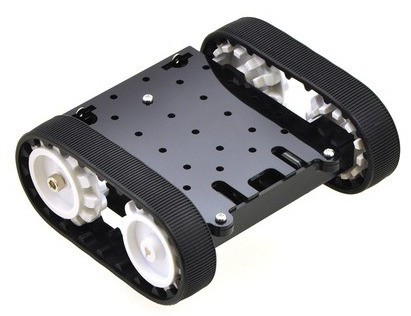
\includegraphics[width=1\textwidth]{images/model_mechaniczny}
  	 \captionof{figure}{Platforma mechaniczna}
     \label{fig:model_mechaniczny}
    \end{subfigure}
    \begin{subfigure}{.45\textwidth}
     \centering
     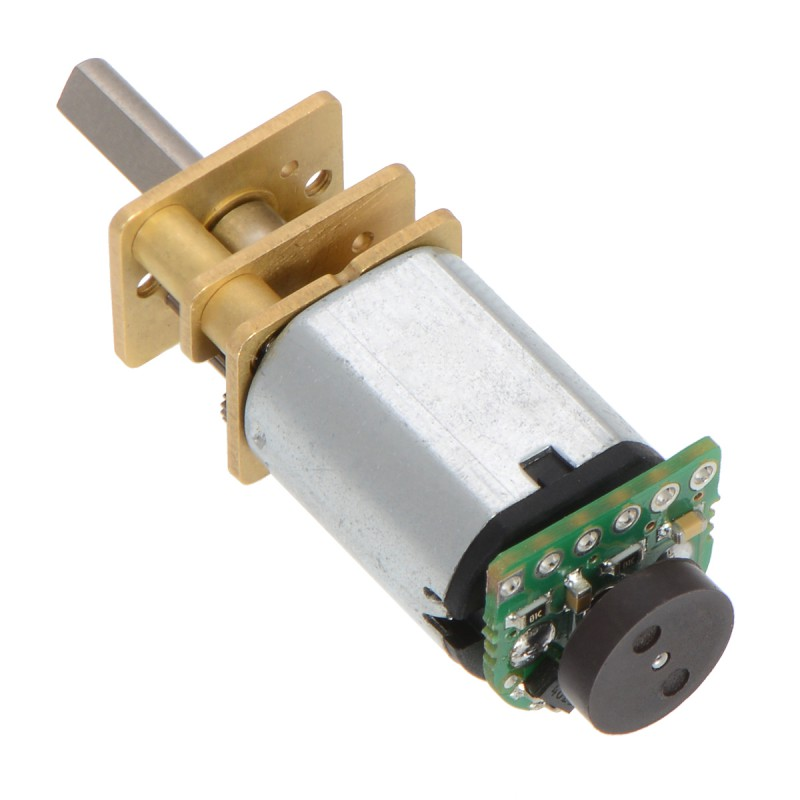
\includegraphics[width=1\textwidth]{images/silnik_enc}
  	 \captionof{figure}{SLinik wrazz enkoderem}
     \label{fig:silnik_enc}
    \end{subfigure}
    \caption{Gotowy moduł nadajnika}
    \label{fig:plytka}
   \end{figure}

Wymiary modelu mechanicznego:
\begin{itemize}
  \item wymiary pełnego modelu: 86[mm] x 98[mm]
  \item odległość pomiędzy kołami (pomiar od środka gąsienicy): 7.5[6mm]
  \item przestrzeń na podstawę elektroniczną:71[mm] x 80[mm]
  \item średnica koła: 1.56[mm]
\end{itemize}

Napędami są miniaturowe silniki Pololu HP z dwustronną osią. Silnik posiada przekładnie 50:1 co ogranicza prędkość obrotową wału silnika zwiększając jednocześnie jego moment. Obustronny wał pozwala na wygodny montaż enkoderów, czyli czujników wykorzystywanych przy pomiarze prędkości obrotowej silnika. Parametry silnika:

\begin{itemize}
  \item Maksymalne napięcie pracy: 9[V]
  \item Prędkość obrotowa dla napięcia 6[V]: 625 obrotów na minutę
  \item Moment obrotowy dla napięcia 6[V]: 1.1 [kg*cm]
  \item Maksymalny prąd dla napięcia 6[V]: 1600[mA]
\end{itemize}

Wybór silnika podyktowany był nie tylko możliwościami jakie oferuje, ale przed wszystkim pełną iteracją z modelem mechanicznym oraz enkoderami (montaż zaprezentowany jest na rysunku powyżej). Dzięki temu konstrukcja była przebiegła szybciej i w dużym stopniu zapobiegła wszelkim błędom montażom. 

 \section{Konstrukcja elektroniczna}
Na konstrukcje elektroniczną robota składają się 4 moduły:
\begin{itemize}
  \item układ Nucleo F401RE z mikrokontrolerem STM32F401
  \item moduł Bluetooth HC-05
  \item zestaw enkoderów magnetycznych 
  \item bazowy obwód łączący układ Nucleo z silnikami 
  \item akumulator LiPol Redox 7.4 V 500mAh
\end{itemize}

  \begin{figure}[ht]
   \centering
   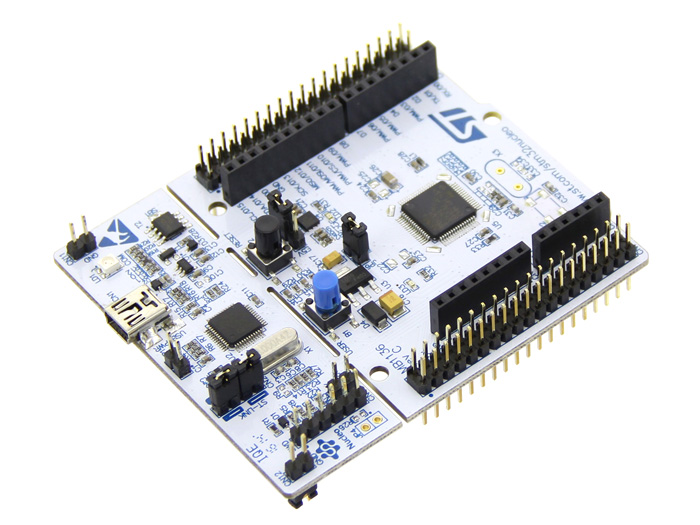
\includegraphics[width=9cm]{images/nucleo}
   \caption{Wizualizacja zasady wyznaczania pozycji}
   \label{fig:nucleo}
  \end{figure} 

Elektronika robota opera się o układ Nucleo F401RE.Sercem układu jest mikrokontroler STM32F401.Posiada on 32-bitową architekturę opartą o rdzeń ARM Cortex M-4 i może być taktowany do 84 MHz. Wydajna jednostka obliczeniowa wraz z sprzętową obsługą operacji na liczbach zmiennoprzecinkowych była kluczowa przy realizacji projektu.  Oprócz szybkiego przetwarzania danych od mikrokontrolera wymagane była sprzętowa realizacja komunikacji szeregowej oraz duża liczba timerów. Obecny mikrokontroler posiada kontroler DMA (ang. Direct Memory Access),pozwalający przeprowadzać transmisję danych bez obciążania procesora, jak również 10 sprzętowych timerów, co pokrywa wymagania projektowanego systemu.
Parametry STM32F401:
\newline Parametry STM32F401:
\begin{itemize}
  \item Częstotliwość taktowania: 84[MHz]
  \item Pamięć trwała Flash: 512kB
  \item Pamięć Static RAM: 96kB
  \item Ilość programowalnych wejść/wyjść: 81
  \item Interfejsy: 3x I2C, 3x USART, 4x SPI, USB 2.0 Full Speed
\end{itemize}

Nie licząc wypowadzeńpinów mikrokontrolera, istotnymi elementami w Nucleo F401RE są stabilizatorynapięcia na 3.3V i 5V z możliwością zasilania bateryjnego od 9V do 12V oraz progrmator/debuger ST-Link v2 . 
\\Komunikacja bezprzewodowa umożliwia moduł HC-05. Techniczne szczegóły opisane są w rozdziale 3.3. Najważniejsze parametry HC-05:
\begin{itemize}
  \item Napięcie zasilania: 3.3[V]
  \item Zasięg: do 10[m]
  \item Komunikacja: UART
  \item Standard: Bluetooth 2.0 + EDR
\end{itemize}

Odczyt prędkości realizowany jest przez enkodery magnetyczneMagnetic Encoder Pair Kit for Micro Metal Gearmotors formy Pololu. Wybór jest wynikał głównie z wyżej wspomnianej integracji z elementami mechanicznymi robota. Podstawą fizyczną działania magnetycznych enkoderów inkrementacyjnych jest efekt Halla.

   \subsection{Bazowy obwód}
   \begin{figure}[ht]
    \centering
    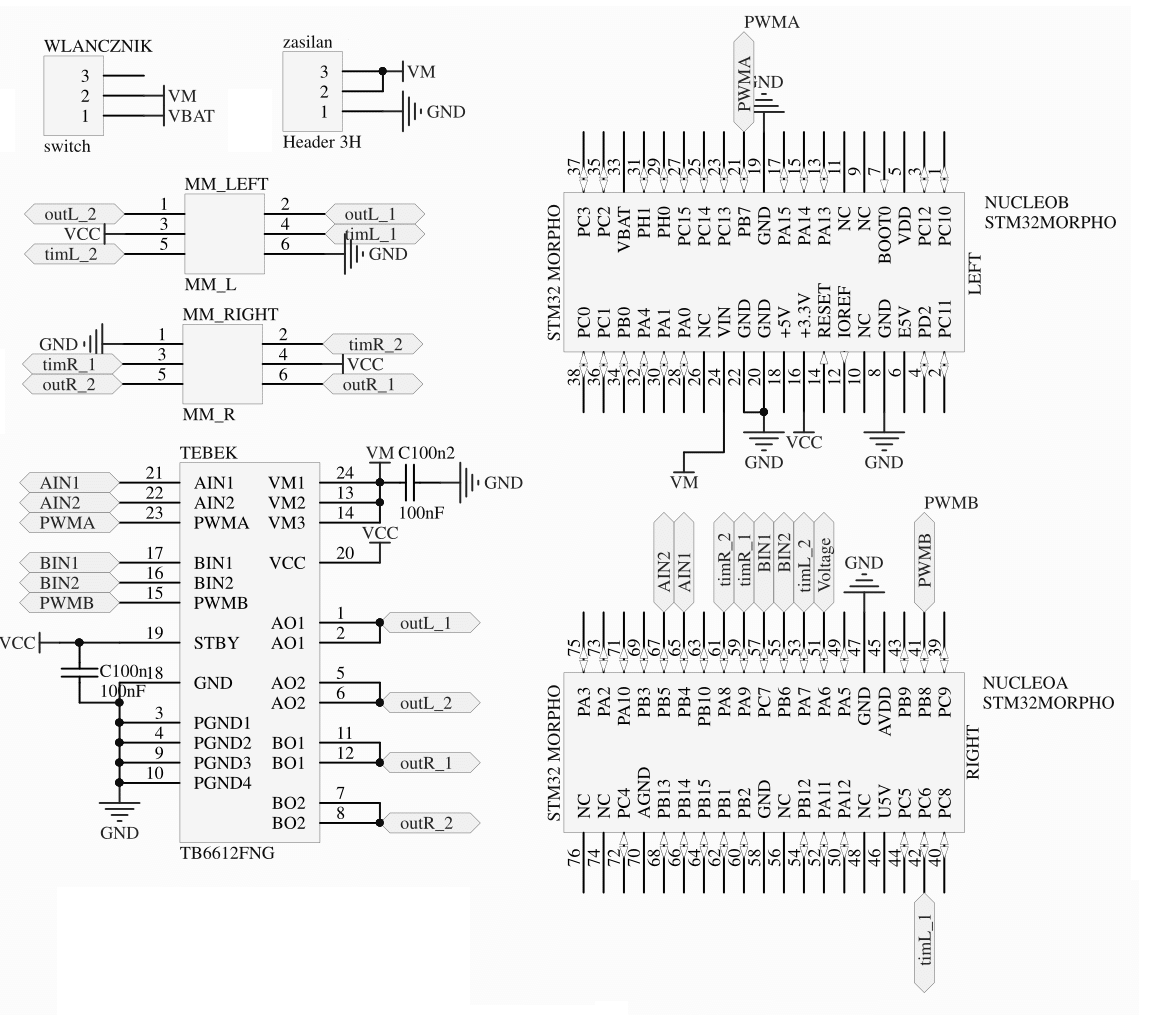
\includegraphics[width=12cm]{images/schemat_elekt}
    \caption{Schemat układu elektronicznego}
    \label{fig:schemat_elekt}
   \end{figure}

Układ elektroniczny zaprojektowany został w programie CircuitMaker firmy Altium. Zadaniem układu było połączenie modułu Nucleo z wyprowadzeniami enkoderami i umieszczenie sterownika silnika. Powszechnym sposobem kontroli silnika prądu stałego jest zastosowanie mostka H. Układ ten pozwala na sterowanie kierunkiem przepływu prądu przez silnik. Funkcja realizowana jest przez układ scalony TB6612FNG, który pozwala na kontrole kierunku obrotów dwóch silników oraz regulacje ich prędkości sygnałem PWM (ang. Pulse Width Modulation). Sygnał zasilający silniki oraz wyprowadzenia enkoderów połączone z układem jest za pośrednictwem złącza micromatch . Wszystkie sygnały podłączone są do mikrokontrolera przez wyprowadzenia Nucelo.
 
\chapter{Oprogramowanie robota mobilnego}
 \section{Struktura oprogramowania}
   \begin{figure}[ht]
    \centering
    \includegraphics[width=1\textwidth]{images/ogol}
    \caption{Schemat blokowy głównego algorytmu robota}
    \label{fig:ogol}
   \end{figure}

Oprogramowanie napisane jest w języku C korzystając z bibliotek HAL (Hardware Abstraction Layer) udostępnionych przez firmę STMicroelectronics. Powyższy schemat pokazuje rozwiązanie podstawowej funkcjonalności robota, czyli regulacji prędkości. Stan robota wyrażonych jest zmiennych globalnych, które poszczególne procedury modyfikują wartość. Cienkie strzałki wskazują kierunek przepływu danych, natomiast grube wskazują na przerwania sprzętowa wyzwalające dane funkcję obsługi. Bezpośrednia zmiana wypełnienia sygnału PWM oraz kierunek obrotu silników za pomocą wiadomości została zaznaczona linią przerywaną. Modyfikacja tych wartości nie jest możliwa podczas trybu regulacji prędkości i wymaga wyłączenia tej procedury( Zagadnienie jest omówione w rozdziale piątym). Przedstawione na schemacie procedury opisane są w dalszej części tego rozdziału. 

 \section{Konfiguracja mikrokontrolera}

Konfiguracja mikrokontrolera wykonana jest przy użyciu oprogramowania STMCubeMX. Pozwala one w bezpieczny i wygony sposób dokonać konfiguracji.

   \begin{figure}[ht]
    \centering
    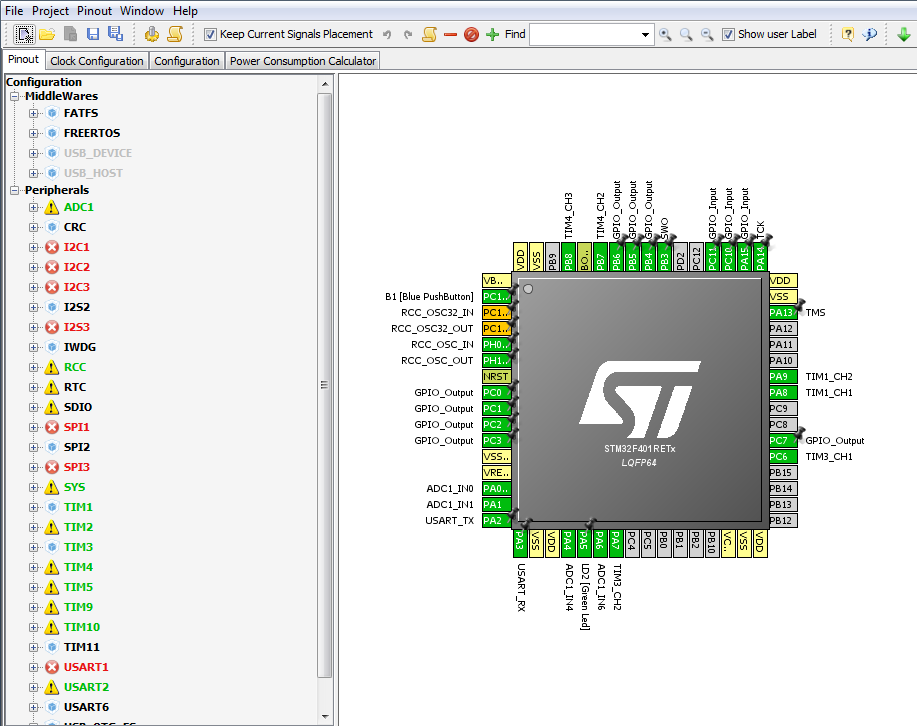
\includegraphics[width=1\textwidth]{images/cubemx1}
    \caption{Konfiguracja pinów mikrokontrolera}
    \label{fig:cubemx1}
   \end{figure}

   \begin{figure}[ht]
    \centering
    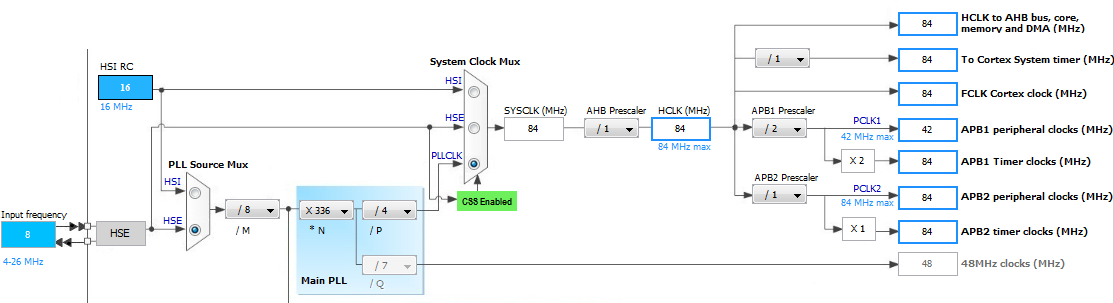
\includegraphics[width=1\textwidth]{images/clock}
    \caption{Konfiguaracja taktowania}
    \label{fig:clock}
   \end{figure}

Mikrokontroler jest taktowany z częstotliwością 84 MHz. Źródłem taktowania jest rezonator kwarcowy 8 MHz, którego częstotliwość jest powielana  przez wewnętrzną pętlę PLL. 

   \begin{figure}[ht]
    \centering
    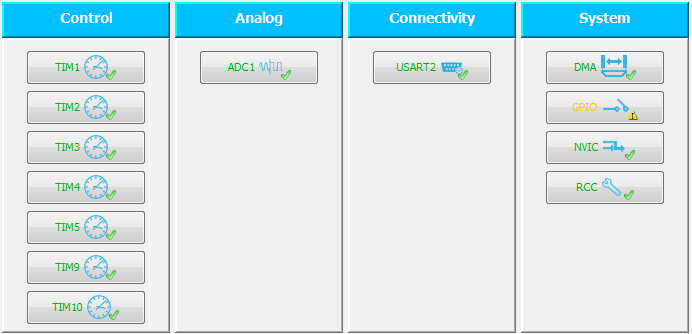
\includegraphics[width=1\textwidth]{images/uC_config}
    \caption{Wykorzystane komponenty STM32F401}
    \label{fig:uC_config}
   \end{figure}

Oprogramowanie wykorzystuje 7 sprzętowych timerów, obsługę transmisji szeregowej UART, magistrale DMA oraz kontroler przerwań NVIC. Oprogramowanie nie zawiera żadnej instrukcji w pętli głównej programu, zachowanie robota jest całkowicie sterowane sprzętowymi przerwaniami. 

 \section{Realizacja komunikacji Bluetooth}

Komunikacja Bluetooth wykorzystuje obsługę dwóch komponentów mikrokontrolera, interfejsu szeregowo UART oraz technika DMA. UART (Universal Asynchronous Receiver and Transmitter) umożliwia asynchroniczne wysyłanie i odbieranie danych przez port szeregowy. Wykorzystanie modułu Bluetooth ogranicza się do połączenia linii danych  TX (wysyłanie) mikrokontrolera z linią danych RX (odbiór) układu HC-06 oraz analogicznie linii RX mikrokontrolera z linią TX modułu. Transmisja bezprzewodowa jest przezroczysta z poziomu mikrokontrolera. Interfejs UART konfigurowany jest przed podanie 4 wartości określających transmisję:
\begin{itemize}
  \item prędkość transmisji (ang. Baud rate)
  \item długość słowa
  \item ilość bitów stopu
  \item bit parzystości (kontrola błędów odbiory danych )
\end{itemize}
Zdecydowałem się na użycie standardowej konfiguracji prędkość: 9600, 8-bitowe słowo, jeden bit stopu, brak bitów parzystości.
\\DMA jest modułem który umożliwia bezpośredni dostęp do pamięci RAM i układów peryferyjnych. Układ DMA umożliwia transfer danych pomiędzy urządzeniem peryferyjnym a pamięcią RAM bez angażowania procesora, którego zadanie ogranicza się do konfiguracji urządzenia. Komponent został użyty do przesyłu i odbioru danych pomiędzy układem UART i dziesięciobajtowym obszarem pamięci RAM. Włączenie odbioru danych szeregowych z użyciem DMA:
\begin{lstlisting}[style=c]
int8_t command[10];
HAL_UART_Receive_DMA(&huart2, command, sizeof(command));
\end{lstlisting}
Argumentami tej funkcji są adres obiektu obsługującego interfejs UART, dziesięciobajtowy obszar pamięci ( tablica dziesięciu bajtów utworzona w globalnej przestrzeni pamięci ) oraz długość tego obszaru. 
\\Asynchroniczność transmisji możliwa jest poprzez obsługę przerwania które generuje UART po zakończeniu transmisji. Biblioteki HAL zapewniają niskopoziomową obsługę przerwań oraz deklaracje zestawu funkcji zwrotnych które zostają wykonane w odpowiedzi na zarejestrowane przerwanie. Obsługa zakończenia transmisji:
\begin{lstlisting}[style=c]
voidHAL_UART_RxCpltCallback(UART_HandleTypeDef *huart)
{
	int8_t response[10];
	int8_t currentCommand[10];
	uint8_t index = 0;
	for(;index < 10; ++index)
		currentCommand[index] = command;
	if(getTimerTimeout(&htim9))
		stopBluetoothTimer();
	commandHandler(currentCommand,response);
	HAL_UART_Transmit_DMA(&huart2,response,10);
	if(getTimerTimeout(&htim9))
		startBluetoothTimer();
}
\end{lstlisting}
Funkcja jest przez bibliotekę HAL wywoływana dla zarejestrowanego przerwania od dowolnego interfejsu UART. Obiekt UART komponentu który wywołał przerwanie jest przekazywany jako argument funkcji. Z uwagi na to, że używany jest jeden interfejs szeregowy nie ma potrzeby sprawdzania czy to on jest źródłem przerwania. Funkcja tworzy tablicę bajtów - response, która wraz z kopią odebranej komendy przekazywana jest do funkcji obsługującej daną wiadomość. Wypełniona odpowiedź wysyłana jest tą samą techniką. Obsługa wiadomości oraz zastosowany timer opisany jest w dalszej części tego rozdziału.
\\Problem, jaki należy rozważyć, w przypadku komunikacji asynchronicznej, jest sytuacja, w której wiadomość jest odbierana zanim wcześniejsza zostanie obsłużona. Dodatkową komplikacja, w tej sytuacji jest użycie DMA, które wypełnia wartości w pamięci z pominięcie pracy, a tym samym kontroli procesora. Praca, na tym samym obszarze pamięci, które wypełnia DMA, podczas obsługi, mogłaby skutkować zmianą wartości tablicy podczas odczytu z niej wiadomości. Z tego powodu, pierwszym etapem w obsłudze przerwania, jest utworzenie kopii tablicy commandi praca na duplikacie. To rozwiązanie, zwiększa stabilność przetwarzania wiadomości, ale nie rozwiązuje problemu całkowicie. Nowa wiadomość mogłaby pojawić się podczas tworzenia duplikatu, co znów generuje ten sam problem. Z pomocą przychodzi tutaj sprzętowa obsługa przerwańw mikrokontrolerach STM. Przetworzenie wiadomości wywoływana jest w obsłudze przerwania, które kończy się dopiero po zaaplikowaniu komendy. Kontroler przerwań NVIC, w przypadku takiego samego priorytetu, tworzy kolejkę LIFO przerwań i a następnie kolejno przekazuje sterowanie, po zakończeniu aktualnie wywołanej funkcji obsługi. Z tego powodu handler nie wywoła się przed zakończeniem przetwarzania bieżącej komendy. Poza wyżej wymienionymi zabezpieczeniami omawiany błąd eliminowany jest przez konstrukcję protokołu komunikacyjnego z aplikacją sterującą. Zgodnie z nim, aplikacja nie wysyła, następnej wiadomości bez otrzymania odpowiedzi na poprzednią, w przypadku prawidłowej wymiany danych, rozwiązuje ten problem.

 \section{Proces przetwarzania wiadomosci}
W poprzednim rozdziale zaprezentowana jest obsługa przerwania od zakończenia transmisji szeregowej. Obecna jest funkcja „commandHandler” odpowiedzialna za obsługę wiadomości i uformowanie odpowiedzi. Struktura  funkcji „commandHandler” ( dla czytelności pominąłem fragment funkcji,n gdyż nie wpływa to na zrozumienie jej działania):
\begin{lstlisting}[style=c]

int8_t* commandHandler(int8_t* command,int8_t* response)
{
if(command[0] != 'B' || command[4] != 'M' || command[9] !='E')
return invalidMessage(response);
if(command[1] == 1)
{
//set speed
returnsetVelocityResponse(command,response);
}
if(command[1] == 2)
{
//get speed
returngetVelocityResponse(command,response);
}
//(...)
if(command[1] == 14)
{
//set direction pins
returnsetMotorsDirection(command,response);
}
if(command[1] == 15)
{
//get direction pins
returngetMotorsDirection(command,response);
}
returninvalidMessage(response);
}
\end{lstlisting}

Działanie prezentowanej funkcji jest ściśle związane z protokołem komunikacyjnym pomiędzy robotem a aplikacją sterującą. Zagadnienie to jest szczegółowo opisane w rozdziale piątym. Początek funkcji sprawdza czy na odpowiednich pozycjach występują wartości stałe i charakterystyczne dla każdej wiadomości, w przeciwnym wypadku wysyłana jest wiadomość informująca o błędzie. Następnie na podstawie identyfikatora wiadomości wywoływana jest konkretna funkcja obsługująca daną wiadomość, a jeżeli podany identyfikator nie jest znany zwracany jest błąd. 
\\Obsługa wiadomości zaprezentowana będzie na przykładzie komendy ustalające prędkość zadaną  w układzie regulacji:
\begin{lstlisting}[style=c]

int8_t* setVelocityResponse(int8_t* command,int8_t* response)
{
uint8_tindex = 0;
for(;index<10; ++index)
response[index] = 0;
response[0] = 'B';
response[1] = command[1];
response[2] = command[2];
response[3] = command[3];
response[4] = command[5];
response[5] = command[6];
if(command[2] == 0 && command[3] == 0 && command[5] == 0 && command[6] == 0)
{
stopMotors();
return response;
}
int8_t data[2];

data[0] = command[2];
data[1] = command[3];
setLeftSpeed = byte2Float(data);

data[0] = command[5];
data[1] = command[6];
setRightSpeed = byte2Float(data);

if(command[7] != 0&& command[8] != 0)
{
data[0] = command[7];
data[1] = command[8];
uint32_t timer = byte2int(data);

startSpeedTimer(timer);
}

return response;
\end{lstlisting}

Działanie prezentowanej funkcji jest ściśle związane z protokołem komunikacyjnym pomiędzy robotem a aplikacją sterującą. Zagadnienie to jest szczegółowo opisane w rozdziale piątym. Początek funkcji sprawdza czy na odpowiednich pozycjach występują wartości stałe i charakterystyczne dla każdej wiadomości, w przeciwnym wypadku wysyłana jest wiadomość informująca o błędzie. Następnie na podstawie identyfikatora wiadomości wywoływana jest konkretna funkcja obsługująca daną wiadomość, a jeżeli podany identyfikator nie jest znany zwracany jest błąd. 
\\Obsługa wiadomości zaprezentowana będzie na przykładzie komendy ustalające prędkość zadaną  w układzie regulacji:
\begin{lstlisting}[style=c]

int8_t* setVelocityResponse(int8_t* command,int8_t* response)
{
uint8_tindex = 0;
for(;index<10; ++index)
response[index] = 0;
response[0] = 'B';
response[1] = command[1];
response[2] = command[2];
response[3] = command[3];
response[4] = command[5];
response[5] = command[6];
if(command[2] == 0&& command[3] == 0&& command[5] == 0&& command[6] == 0)
{
stopMotors();
return response;
}
int8_t data[2];

data[0] = command[2];
data[1] = command[3];
setLeftSpeed = byte2Float(data);

data[0] = command[5];
data[1] = command[6];
setRightSpeed = byte2Float(data);

if(command[7] != 0&& command[8] != 0)
{
data[0] = command[7];
data[1] = command[8];
uint32_t timer = byte2int(data);

startSpeedTimer(timer);
}

return response;
\end{lstlisting}


Każda funkcja początkowo wypełnia odpowiedź zerami i wartościami stałymi. Dla wiadomości typu „ustaw” odpowiedź powinna być identyczna jak komenda przychodząca. Dzięki temu aplikacja sterująca może mieć pewność, że ustawione zostały podane wartości. Pobór fatycznych wartości ustawionych na robocie odbywa się za pomocą wiadomości typu „pobierz”.  Zaprezentowana wiadomość ustawia 3 pozycje: prędkość lewego koła, prędkość prawego koła (w cm/s ) oraz opcjonalnie czas trwania zadanego ruchu. Wiadomości ustawiające prędkość charakteryzują się jeszcze jedną właściwością. Mając wszystkie pola wartości  wypełnione zerami wywołuje się funkcja zatrzymania silników robota. Jest to jedna z form zabezpieczenia. Warunek ten jest sprawdzany od razu po uformowaniu odpowiedzi. Kolejnym etapem jest konwersja odpowiednich bajtów na liczbę zmiennoprzecinkową i zapis wartości do globalnej zmiennej określającej zadaną prędkość dla danego koła. Ostatnim etapem obsługi wiadomości jest ustawienie czasu trwania długości danego ruchu. Jeżeli pola nie są wypełnione zerami wystartuje timer z przesłanymi danymi ilościami milisekund, i po tym czasie zostaną zatrzymane silniki. W przeciwnym razie zadana prędkość będzie się utrzymywała aż do jej zmiany. Po zakończeniu procedury zwracany jest adres z odpowiedzią.

 \section{Zabezpieczenia robota}

Podstawową funkcją wykorzystywaną we każdej formie zabezpieczeń robota jest stopMotors:
\begin{lstlisting}[style=c]
voidstopMotors(void)
{
	setLeftSpeed = 0.0;
	setRightSpeed = 0.0;

	LeftPWM(0);
	RightPWM(0);
	stopSpeedTimer();
}
\end{lstlisting}
Funkcja wyzerowuje wartość zadaną oraz ustawiony PWM, jak również zatrzymuje timer odpowiedzialny za czas trwania ustawionej prędkości. Robot posiada 3 mechanizmy zabezpieczeń. Pierwszym jest wymienione w poprzednim rozdziale wysłanie wiadomości zadającej prędkość z wartościami równymi zero. Kolejnym mechanizmem jest wysłanie niepoprawnej wiadomości. Funkcja przygotowująca odpowiedź informującą o błędzie również zatrzymuje silniki. Ostatnim zabezpieczeniem jest możliwość ustawienia timera Bluetooth ( widoczny jest we fragmencie kodu w podrozdziale 3.2 ). Timer zaczyna odliczanie po otrzymaniu dowolnej wiadomości i gdy następna wiadomość nie pojawi się przed zakończeniem odliczania, silniki są zatrzymywane. Jest to forma zabezpieczenia przed utratą łączności. Domyślnie timer ten jest wyłączony. Włączenie oraz ustalenie czasu odliczania jest możliwe za pomocą wiadomości kontrolnej.

 \section{Realizacja odczytu prędkości}

Aby możliwa była regulacja prędkości wymagane jest sprzężenie zwrotne od faktycznej prędkości osiągniętej przez robota. W tym celu kluczowe jest niezawodne przetwarzanie informacji uzyskanych za pomocą enkoderów. Enkodery zamontowane na wale silników podłączone są to pinów skonfigurowanych jako wejścia kanałów timerów obsługujących ten czujniki. Mikrokontroler STM umożliwia skonfigurowanie timera do trybu Encoder Mode, który wiąże wejście sygnału taktującego licznika z impulsem generowanym przez enkoder. Tryb ten również pozwala na sprzętową analizę kolejności generowanych impulsów wyjściowych, co w wygody sposób pozwala na detekcje kierunku obrotu koła.  (…). Do obliczania prędkości użyty został jeszcze jeden niezależny timer, który o ustawiony interwał aktualizuje globalne zmienne zawierające aktualne prędkości kół robota. 
\begin{lstlisting}[style=c]
voidHAL_TIM_PeriodElapsedCallback(TIM_HandleTypeDef *htim)
{
	if(htim == &htim2)
	{
		leftVelocity = LeftVelocity();
		rightVelocity = RightVelocity();
		htim2.Instance->CNT = encoderTimer - 1;
		HAL_TIM_Base_Start_IT(&htim2);
	}
	//(...)
	else if(htim == &htim3)
	{
		onEncoderOverload(&htim3,&leftTotalTicks);
	}
	Else if(htim == &htim1)
	{
		onEncoderOverload(&htim1,&rightTotalTicks);
	}	
}

\end{lstlisting}
Jest to uniwersalny handler dla wszystkich timerów zarejestrowanych na przerwanie od końca odliczania. Biblioteka HAL obsługuje niskopoziomowo przerwanie timera i wywołuje funkcje obsługi przekazują w argumencie adres obiektu kontrolującego dany licznik. Timer (htim2) odpowiedzialny  za aktualizację prędkości jest obsługiwany na początku zapisuje wyniki funkcji obliczających prędkość oraz zapisuje je zmiennych globalnych. Interwał czasowy dla licznika może być ustalony przez wiadomość kontrolną. Obliczona wartość  jest więc średnią prędkością w ustawionej ramie czasowej.  Z powodu, że interwał aktualizacji prędkości może być ustalany dowolną  szesnastobitową wartością oraz maksymalna prędkość jaką mogą uzyskać koła nie jest stała (zależy od zużycia silników, poziomu naładowania baterii, użytej przekładni i innych czynników ) wymagane było zabezpieczenie przed przekroczeniem maksymalnej wartości timera zanim nastąpi aktualizacja prędkości. Obsługę tej sytuacji zapewnia funkcja:
\begin{lstlisting}[style=c]
void onEncoderOverload(TIM_HandleTypeDef *htim,int32_t *totalTickCounter)
{
if(htim->Instance->CNT >64000&& htim->Instance->CNT <65000)
	*totalTickCounter += (ENCODER_INITIAL + 65000 - htim->Instance->CNT);
else if (htim->Instance->CNT >0&& htim->Instance->CNT <1000)
	*totalTickCounter -= (ENCODER_INITIAL + htim->Instance->CNT);

htim->Instance->CNT = ENCODER_INITIAL;
HAL_TIM_Base_Start_IT(htim);
}

\end{lstlisting}
Argumentami jest adres danego timera oraz adres zmiennej pomocniczej określającej ilość impulsów wysłanych przez enkoder od ostatniej aktualizacji prędkości. Zmienna „totalTickCounter” jest ze znakiem co umożliwia określenie zwrotu prędkości. Prędkość zgodna z przyjętą przednią częścią robota przekracza licznik zmniejszając wartość rejestru przy wartości 0, w związku z czym pod rejestrem, podczas obsługi przerwania,  jest zapisana wartość mniejsza od 65000. Dolne ograniczenie zostało dobrane empirycznie. Analogicznie sytuacja wygląda przy przepełnieniu wartości timera odwrotną prędkością. Zmienna pomocnicza jest inkrementowana lub dekrementowana o obliczoną wartość impulsów.
\\Obliczenie prędkości podczas aktualizacji odbywa się za pomocą funkcji „LeftVelocity” i „RightVelocity”. Obliczanie prędkości koła na przykładzie funkcji „LeftVelocity”:
\begin{lstlisting}[style=c]
floatLeftVelocity(void)
{
leftTotalTicks += (ENCODER_INITIAL -htim3.Instance->CNT);
htim3.Instance->CNT = ENCODER_INITIAL;

float vel = 0.0f;
vel = calcVelocity(leftTotalTicks);
leftTotalTicks = 0;
return vel;
}

\end{lstlisting}

Funkcja dodaje do zmiennej „leftTotalTicks” ilość impulsów wygenerowanych przez enkoder od ostatniej aktualizacji prędkości. Następnie zeruje ilość impulsów, oblicza prędkość liniową w cm/s i zwraca ją. Funkcja obliczająca prędkość liniową:
\begin{lstlisting}[style=c]
floatcalcVelocity(int8_t encoderTicks)
{
float tmp = encoderTicks/TICK_PER_ROUND;
tmp = tmp*2.0*SHORT_PI;
tmp = tmp /(getTimerTimeout(&htim2)*0.0001);
tmp = tmp*RADIUS;
return tmp;
}

\end{lstlisting}

W pierwszym kroku obliczana jest ilość obrotów jakie wykonało koło biorąc po uwagę przekładnie silnika i rozdzielczość samego czujnika . Następnym krokiem jest zamiana ilości obrotów na prędkość kątową wyrażoną w radianach na sekundę. Ostatnim etapem jest uzyskanie prędkości liniowej mnożąc prędkość kątową przez promień koła i zwrócenie wartości.

Przedstawione rozwiązanie jest odporne na duże prędkości,  niemniej jednak może się nie sprawdzać w przypadku małych. Korzystając z enkoderów inkrementalnych należy być świadomym niepewności pomiarowych w odczycie ilości impulsów w stałej ramie czasowej, wywołanej brakiem synchronizacji generowanego przez czujniki sygnału i timera wyzwalającego aktualizację. Problem pogłębia fakt, że sama rama czasowa może być ustalona z zewnątrz podczas pracy robota. Bezpieczniejsze byłoby zablokowanie możliwości zmiany ustawień timera, jednakże byłoby to sprzeczne z ideą projektu. Dobrana empirycznie wartość 60 [ms] jest wartością nominalną i zalecaną podczas korzystania z robota, a za zamianę tej wartości przejmuję pełną odpowiedzialność użytkownik. 

W stałym interwale czasowym problem pojawia wariancja odczytu impulsów, która rośnie wraz ze zmniejszaniem prędkości. Dla stosunkowo dużych prędkości wariancja odczytanych impulsów jest na tyle niewielka, że można ją pominąć, natomiast przy niewielkich potrafi mocno zaburzyć pomiar. W celu wyznaczenia progu prędkości, dla którego pomiar jest stabilny, przygotowany został eksperyment, którego wynika przedstawiono poniżej. Doświadczenie polegało na 30 krotnym pomiarze prędkości oraz ilości impulsów w ramie czasowej dla ustalonego PWM, który następnie inkrementowany był do nowej wartości. W ten sposób wyeliminowano problem błędów wywołanych samym procesem regulacji. 

Pomiar odbył się przy pełnym naładowaniu baterii ( 8.2[V]). Całe doświadczenie było w pełni zautomatyzowane poprzez skrypt JavaScript. W tabeli przedstawione są kolejno: wypełnienie PWM, średnia zliczonych impulsów w ramce  60 ms, ich odchylenie standardowe, procent odcylenia w stosunku do średniej oraz uśredniona prędkość.

\begin{table}[ht]
\centering
\begin{adjustbox}{width=1\textwidth}
\begin{tabular}{ | l | l | l | l | l | }
\hline
	PWM & śr. impulsów & Odchyl. standardowe & Stosunek odch do śr [\%] & Prędkość [cm/s]  \\ \hline
	100 & 6.83 & 0.9 & 13.1412 & 0.7 \\ \hline
	150 & 13.57 & 0.5 & 3.65 & 2.17 \\ \hline
	200 & 19.67 & 0.47 & 2.395 & 3.21 \\ \hline
	250 & 25.3 & 0.86 & 3.407 & 4.26 \\ \hline
	300 & 30.87 & 0.67 & 2.171 & 5.24 \\ \hline
	350 & 36.5 & 0.81 & 2.208 & 6.44 \\ \hline
	400 & 44.33 & 1.08 & 2.425 & 7.82 \\ \hline
	450 & 50.4 & 1.28 & 2.542 & 8.8 \\ \hline
	500 & 56.33 & 1.01 & 1.795 & 9.94 \\ \hline
	550 & 61.93 & 0.57 & 0.927 & 11.07 \\ \hline
	650 & 73.6 & 0.66 & 0.901 & 13.39 \\ \hline
	700 & 80.17 & 0.64 & 0.795 & 14.66 \\ \hline
	800 & 93.6 & 0.5 & 0.534 & 17.15 \\ \hline
	900 & 107.23 & 0.45 & 0.42 & 19.63 \\ \hline
	1000 & 120.93 & 0.47 & 0.389 & 22.12 \\ \hline
\end{tabular}
\end{adjustbox}
\caption{Wyniki doświadczenia} 
\end{table}

Na podstawie widzimy, że odczyt przy prędkości 0,7 cm/s odczyt jest w bardzo dużym stopniu niestabilny o czym świadczą trzynastoprocentowe wahanie w zliczaniu impulsów. Kolejne odczyty odchylenie od średniej, jednakże błąd na poziome 2.5% wciąż może wprowadzić spore oscylacje przy regulacji prędkości. Błąd poniżej 1% uznany został za miarodajny i na podstawie wyników eksperymentu stwierdzona, że pomiar prędkość powyżej 10 cm/s jest stabilny.

 \section{Układ regulacji}
   \begin{figure}[ht]
    \centering
    \includegraphics[width=1\textwidth]{images/regulacja}
    \caption{Schemat układu regulacji}
    \label{fig:regulacja}
   \end{figure}

Bloki o podwójnym obramowaniu oznaczają stan robota, natomiast o pojedynczym reprezentują operację. Strzałki pokazują przepływ danych podczas regulacji prędkości.Uchyb regulacji jest różnicą pomiędzy prędkością zadaną, a aktualną, uzyskaną w trakcie procedury opisanej w poprzedniej sekcji. Wartość uchybu podlega wzmocnieniu i całkowaniu z ustawionymi nastawami, a następnie podlega sumowani ze stanem poprzednim. Operacja ta jest wymagana,  ponieważ sterowniki silników kontrolowane są przez sygnał PWM, nie jest w stanie utrzymać stałej wartości sterującej. To działanie mogłoby być realizowana przez całkujący człon regulatora, jednakże wykorzystane rozwiązanie upraszcza implementacje i dobrze wpasowuje się w dyskretną naturę regulatora.
W implementacji członuróżniczkującego na mikrokontrolerze występuje problem przy dyskretyzacji sygnału. Poniższy wzór aproksymuje operacje różniczkowania na dziedzinie dyskretnej:
\begin{equation}\label{eq:aproksymacja}
   \frac{de(t)}{d} \sim \frac{[e(n) - e(n-1)]}{T} 
  \end{equation}
Pochodna uchybu w systemie dyskretnym przybliżona jest przez iloraz różnicowy. Dokładność wynika przybliżenia jest tym większa, im mniejszy jest okres T. Projekt zakładał wyzwalanie procedury regulacji prędkości poprzez timer, którego interwał ustalany jest wiadomością kontrolną przez użytkownika. Podobnie jak w przypadku aktualizacji prędkości, kosztem poniesionym za swobodę ustawień jest bezpieczeństwo działania układu regulacji. Wartością nominalną timera regulacji jest 150[ms] co jest jednocześnie okresem dyskretyzacji członu różniczkującego. Pomimo, że aproksymacja w te sposób w znaczny sposób od różniczkowania w dziedzinie ciągłej, wykorzystałem to rozwiązanie ze względu na łatwość implementacji oraz jakość regulacji na oczekiwanym poziomie.
\begin{lstlisting}[style=c]
void regulation(void)
{
	eLeft = setLeftSpeed - leftVelocity;
	eRight = setRightSpeed - rightVelocity;
	newPWMLeft = pVal * eLeft + dVal * (eLeft - peLeft);
	newPWMRight = pVal * eRight + dVal * (eRight - peRight) / (getTimerTimeout(&htim10) * 0.0001);         
	peLeft = eLeft;
	peRight = eRight;
	addNewPWM(newPWMLeft,newPWMRight);
}
\end{lstlisting}

Algorytm regulacji zaimplementowany została według wyżej wymienionego sposobu. Okres dyskretyzacji członu różniczkującego przeskalowany został do sekund. Aby regulator działął prawidłowo ważne jest spełnienie warunku:
\begin{equation}\label{eq:aproksymacja}
    T_{regulacji}  \geq  T_{akt. predkosci} 
  \end{equation}
Aktualizacja prędkości musi być odbywać się przynajmniej tak często jak regulacja. W przeciwnym razie, regulator będzie wyliczał uchyb względem błędnej prędkości, co może całkowicie zaburzy pracę robota.

\chapter{Oprogramowanie aplikacji sterującej}
 \section{Struktura oprogramowania}
Aplikacja do sterowania zdalnego robotem została napisana w języka Java. Kod źródłowy jest kompilowany do kodu bajtowego ( forma pośrednia pomiędzy kodem źródłowym, a instrukcjami maszynowymi ) i może być uruchamiany na każdej platformie posiadającej Maszynę Wirtualną Javy. Wybór języka wynika, z wieloplatformowości powstałego programu oraz osobistym doświadczeniu w tworzeniu graficznego interfejsu użytkownika. 

Aplikacja składa się z trzech podstawowych komponentów:
\begin{enumerate}
 \item modułu kontroli komunikacji Bluetooth
 \item modułu sterowania tekstowego
 \item modułu sterowania graficznego
\end{enumerate}

Poza tymi, istnieje jeszcze jeden komponent odpowiedzialny ze utworzenie wyżej wymienionych modułów oraz posiada zbiór funkcji używanych przez wszystkie moduły. Wszystkie komponenty w kodzie źródłowym zorganizowane są w formie pakietów Java. Pakiet Java jest mechanizmem języka, który pozwala grupować powiązane ze sobą klasy, nadając im jednocześnie wspólną przestrzeń nazw.

   \begin{figure}[ht]
    \centering
    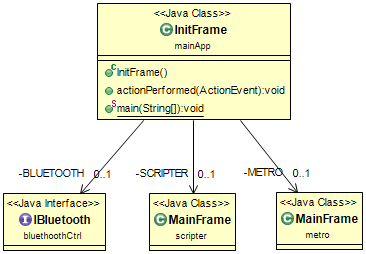
\includegraphics[width=1\textwidth]{images/main}
    \caption{Diagram klas głównego modułu}
    \label{fig:main}
   \end{figure}

Program staruje w klasie głównej InitFrame. Obiekt tej klasy zawiera w sobie egzemplarze klas zarządzających oknami modułów sterujących oraz implementacje interfejsu IBluetooth. Wszystkie przedstawione moduły oraz ich struktura opisane są w dalszej części tego rozdziału. 

 \section{Moduł kontroli komunikacji Bluetooth}

Moduł ten jest komponentem, którego zadaniem jest obsługiwanie transmisji szeregowej Bluetooth z robotem. Moduł definiuje abstrakcyjny interfejs który pozwala na wymianę informacji z robotem, jednocześnie ukrywając techniczne szczegóły realizacji transmisji danych. 

   \begin{figure}[ht]
    \centering
    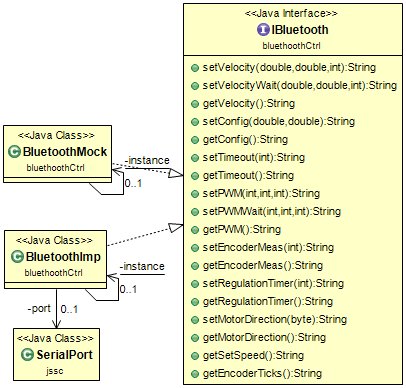
\includegraphics[width=1\textwidth]{images/bt}
    \caption{Diagram klas modułu Bluetooth}
    \label{fig:bt}
   \end{figure}

Podstawą modułu jest interfejs IBluetooth. Udostępnia szereg funkcji, do wymiany danych z robotem. Argumenty funkcji posiadają typ danych, który w naturalny sposób odzwierciedla wartość jaką wyraża. Przykładem może być, zadana prędkość, która posiada typ double, czy czas ekspiracji timera, wyrażony w liczbach całkowitych. Odpowiedzialność za przygotowanie odpowiedniej wiadomości, zgodnej z zaprojektowanym protokołem przeniesiona jest na ten komponent. Warto również zauważyć, że funkcja zadająca prędkość (setVelocity) posługuje się argumentami : Translacja, Rotacja. Z poziomu aplikacji użytkownik korzysta z zadawania prędkości translacji ( ruchu postępowego robota w dwuwymiarowym układzie współrzędnych) i rotacji ( ruchu obrotowego ) , a nie prędkościami poszczególnych kół. Z punktu widzenia użytkownika jest to bardziej intuicyjne rozwiązanie. Pobieranie wartości również jest przekształcane z prędkości lewego i prawego koła na prędkość translacji i rotacji. Transformacje za pomocą funkcji:

\begin{lstlisting}[style=java]
public static double[] TranRot2LeftRight(double translation, double rotation)
{
	double[] result = new double[2] ;
	result[0] = translation + rotation;
	result[1] = translation - rotation;
	return result;
}	
public static double[] LertRight2TranRot(double left,double right)
{
	double[] result =new double[2] ;
	result[0] = (left + right)/2;
	result[1] = (left - right)/2;
	return result;
}

\end{lstlisting}

Każda funkcja zwraca łańcuch znaków zawierająca sformatowaną odpowiedź robota. Wybór tego typu jest omówiony w podrozdziale 4.3.  Interfejs posiada dwie implementacje:

\begin{itemize}
  \item klasa, która symuluje działanie robota, używana we wstępnej fazie implementacji oraz do testowania działania aplikacji bez połączenia z robotem
  \item klasa, która obsługuje połączenie szeregowe poprzez wirtualny port COM z modułem Bluetooth na robocie oraz tworzy właściwe wiadomości gotowe do transmisji
\end{itemize}

Istotną koncepcją przy tworzeniu było zapewnianie, aby tylko jedna instancja obiektu była tworzona podczas pracy programu. Jak w przypadku klasy symulującej nie ma to większego znaczenia, jest niezbędne we właściwej implementacji. Wynika to z faktu, że nawiązywana jest transmisja szeregowa, która blokuje dany port COM. Próba utworzenia kolejnej instancji zakończy się błędem. Rozwiązane to jest poprzez zastosowanie wzorca projektowego singleton. 

Sama obsługa portu szeregowego wykorzystuje bibliotekę jSSC udostępnioną na otwartej licencji. Obsługa portów szeregowych jest ściśle związana z systemem operacyjnym  i wymagana jest ich natywna implementacja, specyficzna dla danego systemu. Zastosowana biblioteka posiada zaimplementowaną natywną obsługę transmisji szeregowej dla większości znanych platform oraz udostępnia abstrakcyjny interfejs w języku Java, który pozwala wykorzystanie go w programie.

 \section{Moduł sterowania tekstowego}
Głównym założeniem przy projektowaniu aplikacji sterującej było umożliwienie użytkownikowi tworzenia skryptów pozwalający implementować dowolny algorytm oraz interakcję z robotem za pomocą komend tekstowych. Wymagało to stworzenie modułu o podstawowej funkcjonalności edytora testowego. Założeniem była również interakcja z poziomu konsoli interpretera, który swoją funkcjonalnością będzie przypominał inne znane interpretery języków skryptowych.

   \begin{figure}[ht]
    \centering
    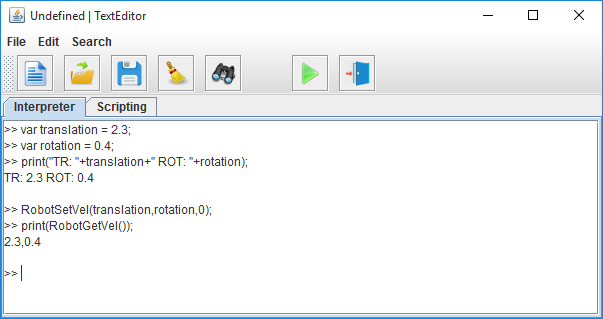
\includegraphics[width=1\textwidth]{images/iterpreter1}
    \caption{Okno panelem interpretera  z interpreterem }
    \label{fig:iterpreter1}
   \end{figure}

Interpreter wykonuje pojedynczą instrukcję, zakończoną średnikiem. Klawisz ENTER rozpoczyna wykonywanie komendy, natomiast klawiszami strzałek możemy przeglądać historie wykonanych instrukcji. Interpreter nie jest związany z panelem sterowania umieszczonym powyżej, interakcja odbywa się tylko za pomocą klawiszy. 

   \begin{figure}[ht]
    \centering
    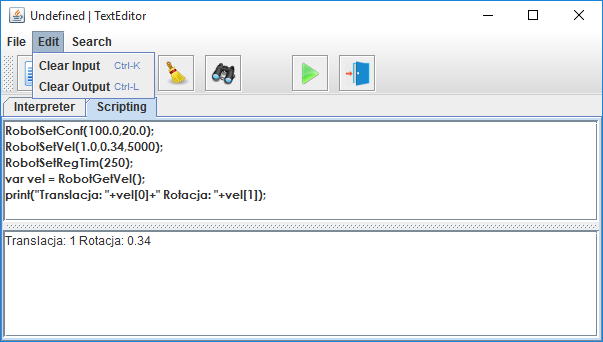
\includegraphics[width=1\textwidth]{images/skryptowanie}
    \caption{Okno z panelem skryptu }
    \label{fig:skryptowanie}
   \end{figure}

Panel edycji skryptów posiada funkcjonalność podstawowego edytora testu. Górne pole tekstowe służy do tworzenia kodu, natomiast dolne jest przekierowanym standardowym wyjściem silnika JavaScript. Powyżej pól tekstowych znajduję się pasek narzędzi oraz menu. Wszystkie funkcje wspomagania edycji dostępne są z poziomu menu, paska narzędzi oraz skrótów klawiszowych. Edytor umożliwia:

\begin{itemize}
 \item uruchomianie skryptu
 \item zapis i odczyt plików z dysku
 \item czyszczenie pola wprowadzania testu i pola wyjściowego
 \item prosty mechanizm przeszukiwania tekstu
 \item zakończenie pracy edytora
\end{itemize}

Ważnym aspektem modułu jest fakt, że zarówno interpreter, jak i edytor korzystają z tej samej instancji silnika JavaScript. Oznacza to, że działania wykonane na jednym panelu widoczne są w drugim. Nie stoi nic na przeszkodzi, aby konfiguracje robota przeprowadzić za pomocą edytora skryptów, natomiast same sterowanie odbyło się za pomocą panelu interpretera.

   \begin{figure}[ht]
    \centering
    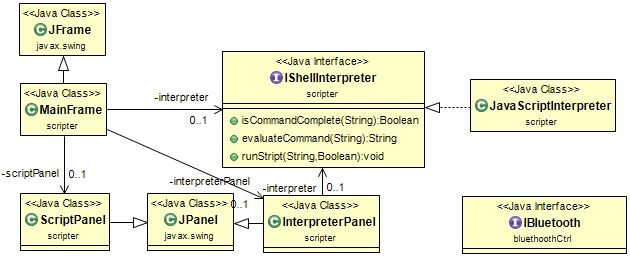
\includegraphics[width=1\textwidth]{images/script}
    \caption{Diagram klas modułu sterowania tekstowego }
    \label{fig:script}
   \end{figure}

Wykorzystanie silnika języka interpretowanego umożliwię interfejs IShellInterpreter. Zastosowanie interfejsu nie wiąże programu z konkretnym silnikiem, umożliwia to w podłączenie dowolnego interpretera bez wprowadzania zmian w programie. Interfejs IBluetooth wywoływany jest poziomu samego JavaScriptu, w związku z czym nie jest powiązany z żadnym z obiektów w module.   

   \subsection{Użycie silnika JavaScript w aplikacji}

Możliwość pisania skryptów wymagała użycia silnika jednego z języków skryptowych. Wybór padł na JavaScript, który główne zastosowanie ma w stronach internetowych. Język ten pozwala na pisanie pełnoprawnych aplikacji oraz realizacji dowolnego algorytmu. Głównym powodem była obecność silnika Nashorn w Java 8 . Jest on wydajną implementacją JavaScript pozwalającą łączyć funkcjonalność obu języków. 

\begin{lstlisting}[style=java]
public class JavaScriptInterpreter implements IShellInterpreter {	
private final String InitialScript="src\\scripter\\cmd.js";
// (...)
private ScriptEngine engine;
// (...)
public JavaScriptInterpreter()
 {
	engine =new ScriptEngineManager().getEngineByName("nashorn");
	stringWriterInit();
	engine.getContext().setWriter(stringWriter);
		
	loadInitScript();		
}
//(...)
\end{lstlisting}

Java 8 udostępnia możliwość stworzenia obiektu klasy ScriptEngine, który zarządza silnikiem JavaScript. Konstruktor obiektu ustawia jako strumień wyjściowy obiekt  tekstowy  stringWriter powiązany z oknem aplikacji oraz uruchamia skrypt początkowy, umieszczając tym samym w przestrzeni JavaScript definicję funkcji używane przy komunikacji z robotem.
Uruchamianie kodu JavaScript
\begin{lstlisting}[style=java]
@Override
public Stringe valuateCommand(Stringcommand) throws ScriptException {
	engine.eval(command);
	String res = stringWriter.toString();
	stringWriter.getBuffer().setLength(0);
	return res;
}
(...)
@Override
public void runStript(Stringtext, Boolean isFromFile) throws Exception{
	stringWriter.setIsEvent(true);
	if(isFromFile)
		engine.eval(newFileReader(text));
	else
		engine.eval(text);
	stringWriter.setIsEvent(false);
		
}

\end{lstlisting}
Przedstawione metody używane są przy wywoływaniu skryptów. Pierwsza funkcja używana jest przez panel interpretera. Po wykonaniu fragmentu kodu ( „engine.eval(command);”)czyści bufor a następnie umieszcza w nim dane odebrane z standardowego wyjścia silnika. Druga funkcja używana jest w edytorze skryptów. Pozwala na uruchamianie zarówno plików tekstowych jak i ciągów znaków. W tej metodzie przekierowanie strumienia wyjściowego opiera się na obsłudze generowanych prze obiekt stringWriter  zdarzeń.

Fragment inicjalnego skryptu umożliwiającego kontakt z robotem:
\begin{lstlisting}[style=java]
var BluethoothClass = Java.type('bluethoothCtrl.BluetoothImp');
var btObject = BluethoothClass.getInstance();
//(...)
function RobotSetVel(translate,rotate,time)
{
	var result =btObject.setVelocity(translate,rotate,time);
	returndecode(result);
}
function RobotGetVel()
{
	var result = btObject.getVelocity();
	returndecode(result);
}
//(...)
\end{lstlisting}

Sam inicjalny skrypt ładowany podczas konstruktora klasy opakowuje wszystkie metody interfejsu IBluethooth. Skrypt uzyskuję dostęp do klasy Java ( jedna z wspomnianych wcześniej możliwości silnika Nashorn ) oraz pobiera statyczny obiekt tej klasy. Każda funkcja wywołuje metodę z interfejsu  IBluethoot, a następnie zwraca zdekodowany do tablicy łańcuch znaków. Powodem, dla którego w interfejsie IBluethooth każda metoda zwraca ten typ jest fakt, że z poziomu JavaScript pobieranie zmiennej tekstowej działa zawsze zgodnie z oczekiwaniami, czego nie można powiedzieć o innych typach danych.

 \section{Moduł sterowania graficznego}

Wykorzystanie potencjału sterowanie tekstowego wymaga podstawowej wiedzy programistycznej i poświęcenia czasu aby w pełni poprawnie przygotować skrypt. Poza tym moduł ten nadaje się do implementacji algorytmu poruszania się robota, niekoniecznie natomiast sprawdza się w sytuacji gdy chcemy , aby robot reagował na nasze działania w czasie rzeczywistym. Odpowiedzią  na ten problem jest moduł sterowania graficznego. Idea tego komponentu polega na wykorzystaniu bloków sterujących, które pozwalająca komunikację z robotem za pomocą interfejsu graficznego. Bloki sterujące pozwalają na zmianę konfiguracji robota, kontrolę  i wizualizację prędkości bez konieczności używanie komend tekstowych. 

Główne okno modułu graficznego pozwala wybierać bloki, które chcemy aktualnie użyć przy sterowaniu robotem, spośród wszystkich dostępnych. Dodatkowo w menu umieszczone są dwie pomocnicze opcje pozwalające na dodawanie bądź usunięcie wszystkich bloków. Bloki sterujące są szczegółowo opisane w następnych podrozdziałach.

\begin{center}
  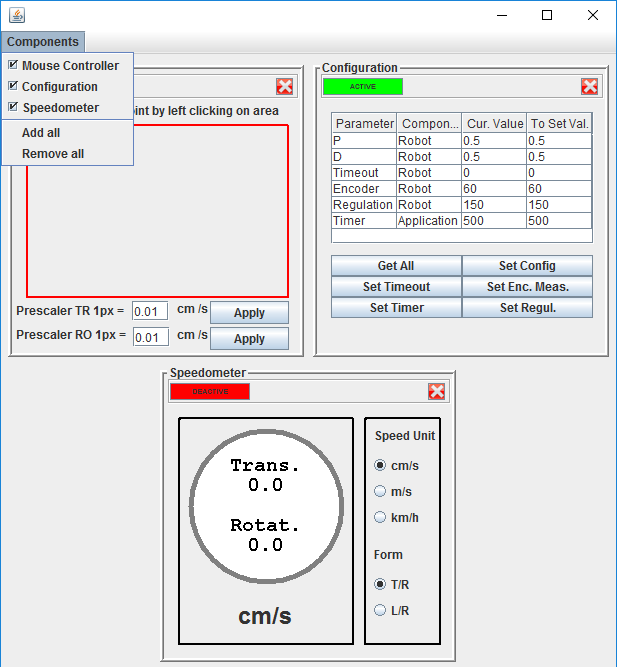
\includegraphics{images/metro_all}
  \captionof{figure}{Okno modułu graficznego}
\end{center}

Samo okno aplikacji pozwala dynamicznie zarządzać blokami na ekranie. W zależności od rozmiaru okna bloki układają się w sposób, aby jak najefektywniej wykorzystać dostępną przestrzeń. Rozkład elementów można kontrolować poprzez kolejność dodawania bloków do głównego okna. Minimalizacja i zamknięcia okna wysyłają komendę stop do robota.

 \subsection{Bazowy blok sterujący}

\begin{center}
  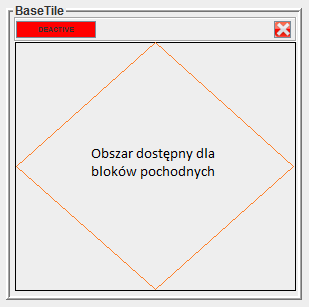
\includegraphics{images/bazowy}
  \captionof{figure}{Bazowy blok sterujący}
\end{center}

Przycisk z krzyżykiem odpowiada za wyłączenie elementu i jest jednoznaczny z odznaczeniem elementu w głównym oknie modułowym. Przycisk aktywacji określa włączenie działania bloku i jest podstawowym mechanizmem w synchronizacji pracy. Współpraca bloków opisana jest w podrozdziale 4.4.3. Ich wymiary  są ustalone i nie podlegają modyfikacji. Blok może modyfikować udostępnione przez klasę BaseTile ciało elementu.

Właściwości wspólne dla każdego elementu :
\begin{itemize}
  \item nazwa – każdy blok musi wprowadzić swoją unikalną nazwę
  \item typ  - blok może by jednego z trzech typów
  \begin{itemize}
    \item STEROWANIE – element kontrolujący ( zadający) prędkość robota
    \item WIZUALIZACJA – element wizualizujący faktyczną prędkość robota
    \item KONFIGURACJA – element, który nie steruje prędkością, może natomiast zmieniać konfiguracje robota np. nastawy regulatora
  \end{itemize}
  \item definiuje podstawową funkcję aktywacji i dezaktywacji elementu. Element może rozszerzyć tą funkcjonalność, niemniej jednak musi wtedy wywołać funkcje klasy bazowej
  \item definiuje funkcje wyłączenia elementu
\end{itemize}

\begin{center}
  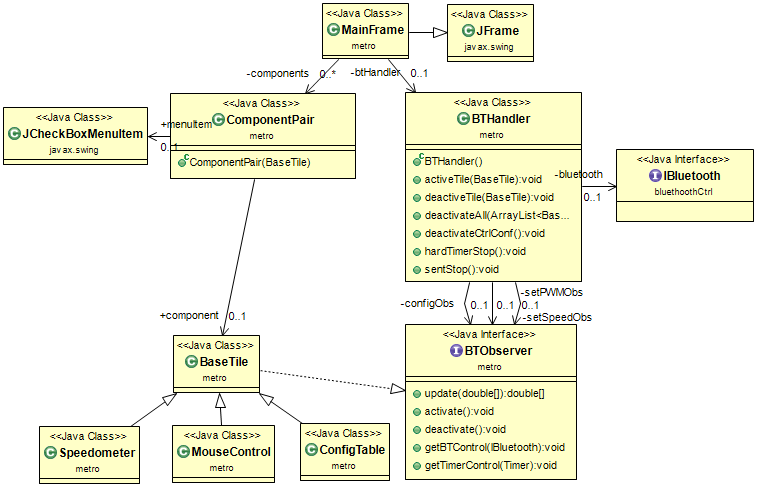
\includegraphics{images/metro}
  \captionof{figure}{Diagram klas modułu sterowania graficznego}
\end{center}

Obiekt skojarzony z głównym oknem modułu zawiera listę obiektów ComponentPair łączących bloki sterujące oraz pola wyboru. Życiem obiektów implementujących zarządza obiekt głównej klasy. Kolejnym komponentem jest obiekt klasy BTHandler kieruje komunikacją pomiędzy modułem Bluetooth  a blokami sterującymi oraz jest odpowiedzialny za synchronizację pracy bloków sterujących. Klasa ta uzyskuje referencję do obiektów sterujących i komunikuje się z nimi przez interfejs BTObserver. Działanie poszczególnych bloków oraz synchronizacja ich pracy opisana jest w dalszej części rozdziału.

\newpage
\subsection{Bloki sterujące dostępne w aplikacji}

W aplikacji stworzone zostały 3 bloki sterujące, po jednym w każdym typie. 

\begin{description}
  \item[Nazwa] Sterowanie Myszką
  \item[Typ] STEROWANIE
\end{description}

   \begin{figure}[ht]
    \centering
    \begin{subfigure}{.45\textwidth}
     \centering
     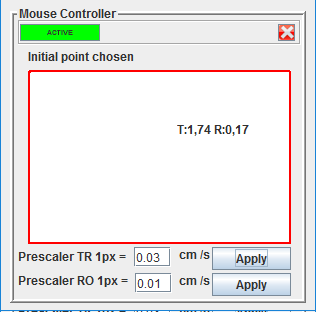
\includegraphics[width=1\textwidth]{images/mause1}
     \label{fig:mause1}
    \end{subfigure}
    \begin{subfigure}{.45\textwidth}
     \centering
     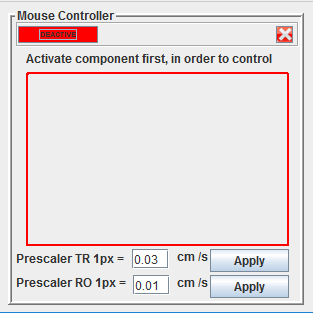
\includegraphics[width=1\textwidth]{images/metro2}
     \label{fig:metro2}
    \end{subfigure}
    \caption{Sterowanie myszką}
    \label{fig:Blok_ster}
   \end{figure}

Blok umożliwia zadawanie prędkości za pomocą myszki. W centralnej części elementu znajduje się obszar obramowany czarowną linią i główny panel sterowania. Naprowadzenie kursora spowoduje zmianę koloru z szarego na biały, natomiast kliknięcie myszką rozpocznie sterowanie. Po rozpoczęciu sterowania nad kursorem pojawi się napis określający zadaną prędkość translacji i rotacji robota wyrażony w cm/s. Punkt zerowy jest w miejscu kliknięcia, które rozpoczyna sterowanie robotem. Na głównym panelem znajduje się informator aktualnego stanu bloku. Pod głównym panelem jest możliwość ustawienia przeskalowania ruchu myszki ( zmiana o ilości pikseli ) na zadaną prędkość. Praktyka pokazuje, że lepiej steruje się robotem, gdy przeskalowanie translacji jest większe niż rotacji.  Przesunięcie myszki w pionie zmienia rotację, natomiast przesunięcie w poziomie zmienia zadaną rotację. Można zadawać prędkości zarówno dodatnie jak i ujemne. Ponowne kliknięcie, bądź wyjście kursora poza panel główny powoduje zakończenie sterowania.
\newpage
\begin{description}
  \item[Nazwa] Prękościomierz
  \item[Typ] WIZUALIZACJA
\end{description}

   \begin{figure}[ht]
    \centering
    \begin{subfigure}{.45\textwidth}
     \centering
     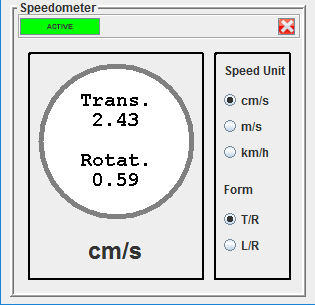
\includegraphics[width=1\textwidth]{images/speed1}
     \label{fig:speed1}
    \end{subfigure}
    \begin{subfigure}{.45\textwidth}
     \centering
     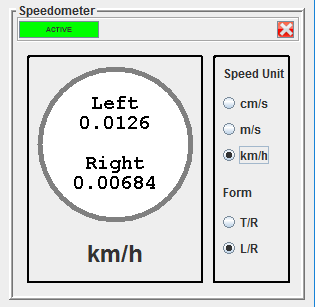
\includegraphics[width=1\textwidth]{images/speed2}
     \label{fig:speed2}
    \end{subfigure}
    \caption{Blok prędkościomierza}
    \label{fig:blok_wiz}
   \end{figure}

Prędkościomierz pokazuje aktualną prędkość robota. Lewy panel odpowiada za wyświetlenie prędkości natomiast prawy za formę w jakiej prędkość ma być wyświetlana. Za pomocą prędkościomierza może ustawić jednostkę w jakiej chcemy prezentować  prędkość:
\begin{itemize}
 \item centymetry na sekundę(domyślnie)
 \item metry na sekundę 
 \item kilometry na godzinę
\end{itemize}
Kolejną opcją jest ustawienie formy wyświetlenia prędkości:
\begin{itemize}
 \item prędkość translacji i rotacji robota ( domyślnie)
 \item prędkość lewego i prawego koła robota
\end{itemize}

\newpage
\begin{description}
  \item[Nazwa] Konfiguracja
  \item[Typ] KONFIGURACJA
\end{description}

   \begin{figure}[ht]
    \centering
    \begin{subfigure}{.45\textwidth}
     \centering
     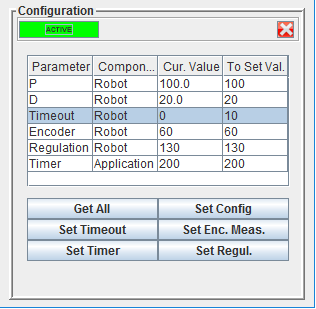
\includegraphics[width=1\textwidth]{images/conf1}
     \label{fig:conf1}
    \end{subfigure}
    \begin{subfigure}{.45\textwidth}
     \centering
     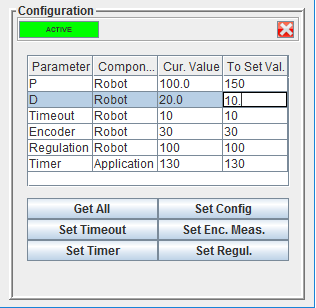
\includegraphics[width=1\textwidth]{images/conf2}
     \label{fig:conf2}
    \end{subfigure}
    \caption{Konfiguracja robota}
    \label{fig:Blok_ster}
   \end{figure}

Prędkościomierz pokazuje aktualną prędkość robota. Lewy panel odpowiada za wyświetlenie prędkości natomiast prawy za formę w jakiej prędkość ma być wyświetlana. Za pomocą prędkościomierza może ustawić jednostkę w jakiej chcemy prezentować  prędkość:
\begin{itemize}
 \item parametr (pierwsza kolumna) : określa ustawionyparametr
 \item komponent (druga kolumna) : określa czy dany parametr dotyczy konfiguracji robota czy aplikacji 
 \item aktualna wartość (trzecia kolumna):pokazuje aktualnie ustawiony parametr
 \item wartość do ustawienie(czwarta kolumna):jedyna  gdzie pola można modyfikować. Pozwala na wpisanie wartości, którą będziemy mieli możliwość ustawić
\end{itemize}
Kolejną opcją jest ustawienie formy wyświetlenia prędkości:
\begin{itemize}
 \item ustawianie timera zabezpieczającego przed utratą łączności Bluetooth ( Timeout)
 \item ustawianie timera aktualizacji prędkości(Encoder) oraz interwału regulatora(Regulation)
 \item ustawienie timera modułu graficznego (Timer) , omówiony szczegółowo w podrozdziale 4.4.3
\end{itemize}

\newpage
  \subsection{Synchronizacja aktywności bloków}

Architektura blokowa modułu graficznego pozwala na tworzenie nieograniczonej ilości bloków sterujących dowolnie wybranego typu. Kontrolowanie prędkości robota może być, oprócz sterowania myszką realizowane przez klawiaturę, joystick czy nawet komendy głosowe. Konfigurowanie robota również może przyjmować wiele różnych form. Z tego powodu wymagane było wprowadzenie mechanizmu synchronizacji pracy bloków. Klasa, która odpowiada za zarządzanie blokami sterującymi jest  wspomniany już BTHandler. Oprócz synchronizacji klasa ta bierze odpowiedzialność za kontrolowanie  dostępu do komponentu Bluetooth dla bloków funkcyjnych.  

Podstawowym elementem, służącym synchronizacji jest przytoczony wcześniej mechanizm aktywacji. Aby działanie komponentu było możliwe, musi być on aktywowany. Uruchomienie elementu następuje w dwóch etapach. Pierwszy jest w obszarze obiektu klasy BTHandler. Obiekt posiada informacje o wszystkich blokach w aplikacji i aktywowanie komponentów podlega niżej wymienionym zasadom:

\begin{itemize}
 \item aktywny może być tylko jeden komponent typu STEROWANIE lub KONFIGURACJA. Uruchomienie więcej niż jednego komponentu tego typu powoduje dezaktywacje bloku aktualnie pracującego
 \item aktywnych może być dowolna ilość bloków typu WIZUALIZACJA
 \item timer modułu graficznego rozpoczyna odliczanie gdy przynajmniej jeden komponent typu STEROWANIE lub WIZUALIZACJA jest aktywny, a wyłącza się gdy nie jest aktywny żaden z tych elementów
 \item wyłączenie elementu powoduje jego automatyczną dezaktywację
 \item minimalizacja lub wyłączenie okna powoduje dezaktywację wszystkich elementów
\end{itemize}

Drugi etap aktywacji realizowany jest w przestrzeni danego bloku i przygotowuje go do pracy. Wymiana danych  bloków typu STEROWANIE  i WIZUALIZACJE jest  cyklicznie uruchamiana przez, wymieniony już wcześniej,  timer aplikacyjny. Licznik ten co podany okres uruchamia swoją funkcję obsługi:

\begin{lstlisting}[style=java]
Private class Task implements ActionListener
{
private int currentVal =0;
private const int typeNumber = 1; 
double[] velocity;
		
private void iterate CurrentVal()
{
	if(currentVal != typeNumber)
		currentVal++;
	else
		currentVal =0;
}
		
@Override
public void actionPerformed(ActionEvent e) {
try{	
	if(setSpeedObs !=null && currentVal ==0)
	{
		velocity = setSpeedObs.update(null);
		bluethooth.setVelocity(velocity[0], velocity[1], 0);
		System.out.println("SET Tr: "+velocity[0]+" Rot: "+ velocity[1]);
	}
	if(!getSpeedObs.isEmpty() && currentVal ==1)
	{
		String tmp = bluethooth.getVelocity();
		velocity =GeneralConverter.deserializeStr2Dbl(tmp);
		System.out.println("GET Tr: "+velocity[0]+" Rot: "+ velocity[1]);
		for(BTObserver obs : getSpeedObs)
			obs.update(velocity);
	}
				
	}catch(SerialPortException serial E) {}
		System.err.println("Bluetooth transmission error!!!");	
	}
}
\end{lstlisting}
Obsługa przepełnienia timera naprzemienne aktualizuje włączony blok sterujący i  wszystkie bloki pobierające aktualną prędkość.

\chapter{Protokół komunikacyjny}  

Protokół komunikacyjny używany do wymiany danych pomiędzy robotem, a aplikacją składa się z 15 wiadomości kontrolnych. Wiadomości pozwalają  pobierać i ustawiać dane na robocie. W większości występują w parach ustaw/pobierz. Protokół nie zakłada istnienia wiadomości jednocześnie zmieniających stan robota i pobierających aktualny stan. Prawidłowa odpowiedź na komendę typu ustaw jest identyczna do odebranej komendy, natomiast obsługa wiadomości typu pobierz nie ujmuje pod uwagę pól danych odebranej komendy.

Wiadomość składa się z 10 bajtów:
\begin{table}[!htb]
\centering
\begin{adjustbox}{width=1\textwidth}
\label{my-label}
\begin{tabular}{|l|l|l|l|l|l|l|l|l|l|l|}
\hline
Nr bajtu          & 0   & 1  & 2    & 3    & 4   & 5    & 6    & 7    & 8    & 9   \\ \hline
Rodzaj wiadomości & "B" & ID & Dane & Dane & "M" & Dane & Dane & Dane & Dane & "E" \\ \hline
\end{tabular}
\end{adjustbox}
\end{table}

Bajty 0, 4 i 9 w każdej wiadomości  są stałe i są równe wartości danej litery w kodzie ASCII. Służą one do kontroli poprawności przesłanej wiadomości.

Bajt 1 określa identyfikator danej wiadomości i na jego podstawie oprogramowanie robota jest w stanie uruchomić odpowiednią funkcję obsługi przesłanej wiadomości. Zostało to zaprezentowane w rozdziale 3.4.

Reszta bajtów przenosi dane konkretnej wiadomości. Wiadomości pozwalają na kodowanie liczby zmiennoprzecinkowej, jak również większych niż 1 bajt liczb całkowitych.

 \section{Spis wiadomości kontrolnych}   

Każda wiadomość kontrolna przedstawiona jest według poniższego schematu:
\begin{table}[!htb]
\centering
\begin{adjustbox}{width=1\textwidth}
\label{my-label}
\begin{tabular}{|l|l|l|l|l|l|l|l|l|l|}
\hline
\multicolumn{4}{|l|}{Nazwa Wiadomości} & \multicolumn{4}{l|}{Komenda Javascript} & \multicolumn{2}{l|}{Typ} \\ \hline
BAJT 0      & BAJT 1      & BAJT 2     & BAJT 3      & BAJT 4      & BAJT 5      & BAJT 6      & BAJT 7     & BAJT 8     & BAJT 9     \\ \hline
\multicolumn{10}{|c|}{CHARAKTERYSTKA WIADMOSCI}                                                                                       \\ \hline
\end{tabular}
\end{adjustbox}
\end{table}

Dla wielkości USTAW w drugim wierszu zaprezentowana jest komenda którą odbiera robot, dla wiadomości typu POBIERZ jest to odpowiedź otrzymywana przez aplikację sterującą.

\begin{table}[!htb]
\centering
\begin{adjustbox}{width=1\textwidth}
\label{my-label}
\begin{tabular}{|c|c|c|c|c|c|c|c|c|c|}
\hline
\multicolumn{4}{|l|}{Ustawienie prędkości zadaniej} & \multicolumn{4}{l|}{RobotSetVel(float TR,float ROT,float time)} & \multicolumn{2}{l|}{USTAW} \\ \hline
"B" \hspace{1em}             & 1\hspace{2em}              & L1\hspace{2em}              & L2\hspace{2em}         & "M"\hspace{2em}         & R1\hspace{2em}         & R2\hspace{2em}         & T1\hspace{2em}         & T2\hspace{2em}          & "E"\hspace{2em}          \\ \hline
\end{tabular}
\end{adjustbox}
\end{table}
Wiadomość ustawia prędkość zadaną dla regulatora. 
Wartości L1 i L2 są zserializowaną zmienną zmiennoprzecinkową oznaczającą zadaną prędkość dla lewego koła
Wartości R1 i R2 są zserializowaną zmienną zmiennoprzecinkową oznaczającą zadaną prędkość dla prawego koła 
Wartości T1 i T2 są rozłożoną 16-bitową zmienną całkowitą oznaczającą ilość milisekund po jakim zadana prędkość" będzie wyzerowana. 
Jeżeli wartość T1 i T2 wynoszą zero timer odpowiedzialny za zatrzymanie silników po ustalonej wartości nie będzie uruchomiony a zadana prędkość nie będzie zmieniana.

Dane zawierające prędkości są deserializowane i zapisywane do odpowiadających im globalnych zmiennych robota. Jeżeli te dane zawierają wszystkie wartości równe zero silniki są zatrzymywane
Wywołując komendę z poziomu JavaScript prędkoć translacji i rotacji zamieniana jest na lewego i prawego koła przed wysłaniem.
Komenda zwraca sterowanie od razu po wywołaniu

\begin{table}[!htb]
\centering
\begin{adjustbox}{width=1\textwidth}
\label{my-label}
\begin{tabular}{|c|c|c|c|c|c|c|c|c|c|}
\hline
\multicolumn{4}{|l|}{Ustawienie prędkości zadaniej z blokadą} & \multicolumn{4}{l|}{RobotSetVelWait(float TR,float ROT,float time)} & \multicolumn{2}{l|}{USTAW} \\ \hline
"B" \hspace{1em}             & 17\hspace{2em}              & L1\hspace{2em}              & L2\hspace{2em}         & "M"\hspace{2em}         & R1\hspace{2em}         & R2\hspace{2em}         & T1\hspace{2em}         & T2\hspace{2em}          & "E"\hspace{2em}          \\ \hline
\end{tabular}
\end{adjustbox}
\end{table}

Komenda różni się od poprzedniej tym, że zwraca sterowanie po ekspiracji timera

\begin{table}[!htb]
\centering
\begin{adjustbox}{width=1\textwidth}
\label{my-label}
\begin{tabular}{|c|c|c|c|c|c|c|c|c|c|}
\hline
\multicolumn{4}{|l|}{Pobranie faktycznej prędkości } & \multicolumn{4}{l|}{RobotGetVel()} & \multicolumn{2}{l|}{POBIERZ} \\ \hline
"B" \hspace{1em}             & 2\hspace{2em}              & L1\hspace{2em}              & L2\hspace{2em}         & "M"\hspace{2em}         & R1\hspace{2em}         & R2\hspace{2em}         & 0\hspace{2em}         & 0\hspace{2em}          & "E"\hspace{2em}          \\ \hline
\end{tabular}
\end{adjustbox}
\end{table}

Wiadomość zwraca faktyczną prędkość, jaką posiada robot. 
Wartości L1 i L2 są zserializowaną zmienną zmiennoprzecinkową oznaczającą faktyczną prędkość dla lewego koła
Wartości R1 i R2 są zserializowaną zmienną zmiennoprzecinkową oznaczającą faktyczną prędkość dla lewego koła 

Odsyłane prędkości są zserializowanymi zmiennymi globalnymi, których wartość obliczana  jest w cyklu aktualizacji prędkości. Opis procedury jest w rozdziale 3.5

\begin{table}[!htb]
\centering
\begin{adjustbox}{width=1\textwidth}
\label{my-label}
\begin{tabular}{|c|c|c|c|c|c|c|c|c|c|}
\hline
\multicolumn{4}{|l|}{Ustawienie nastaw regulatora } & \multicolumn{4}{l|}{setConfig(double P, double D)} & \multicolumn{2}{l|}{USTAW} \\ \hline
"B" \hspace{1em}             & 3\hspace{2em}              & P1\hspace{2em}              & P2\hspace{2em}         & "M"\hspace{2em}         & D1\hspace{2em}         & D2\hspace{2em}         & 0\hspace{2em}         & 0\hspace{2em}          & "E"\hspace{2em}          \\ \hline
\end{tabular}
\end{adjustbox}
\end{table}

Wiadomość ustawia nastawy regulatora. 
Wartości P1 i P2 są zserializowaną zmienną zmiennoprzecinkową oznaczającą wartość wzmocnienia członu proporcjonalnego regulatora PD
Wartości P1 i P2 są zserializowaną zmienną zmiennoprzecinkową oznaczającą wartość wzmocnienia członu różniczkującego regulatora PD

Dane są deserializowane i zapisywane do odpowiadających im globalnych zmiennych robota.

\begin{table}[!htb]
\centering
\begin{adjustbox}{width=1\textwidth}
\label{my-label}
\begin{tabular}{|c|c|c|c|c|c|c|c|c|c|}
\hline
\multicolumn{4}{|l|}{Pobranie nastaw regulatora  } & \multicolumn{4}{l|}{getConfig()} & \multicolumn{2}{l|}{POBIERZ} \\ \hline
"B" \hspace{1em}             & 4\hspace{2em}              & P1\hspace{2em}              & P2\hspace{2em}         & "M"\hspace{2em}         & D1\hspace{2em}         & D2\hspace{2em}         & 0\hspace{2em}         & 0\hspace{2em}          & "E"\hspace{2em}          \\ \hline
\end{tabular}
\end{adjustbox}
\end{table}
 Wiadomość zwraca aktualne nastawy regulatora. 
Wartości P1 i P2 są zserializowaną zmienną zmiennoprzecinkową oznaczającą wartość wzmocnienia członu proporcjonalnego regulatora PD
Wartości P1 i P2 są zserializowaną zmienną zmiennoprzecinkową oznaczającą wartość wzmocnienia członu różniczkującego regulatora PD

Odsyłane nastawy  są zserializowanymi zmiennymi globalnymi.


\begin{table}[!htb]
\centering
\begin{adjustbox}{width=1\textwidth}
\label{my-label}
\begin{tabular}{|c|c|c|c|c|c|c|c|c|c|}
\hline
\multicolumn{4}{|l|}{Ustawienie timera bezpieczeństwa } & \multicolumn{4}{l|}{setTimeout(int timeout)} & \multicolumn{2}{l|}{USTAW} \\ \hline
"B" \hspace{1em}             & 5\hspace{2em}              & T1\hspace{2em}              & T2\hspace{2em}         & "M"\hspace{2em}         & 0\hspace{2em}         & 0\hspace{2em}         & 0\hspace{2em}         & 0\hspace{2em}          & "E"\hspace{2em}          \\ \hline
\end{tabular}
\end{adjustbox}
\end{table}

Wiadomość ustawia timer bezpieczeństwa. Timer jest startuje wraz z odebraniem wiadomości przez robota. Jeżeli nie otrzyma następnej wiadomości przed końcem odliczania robot zatrzyma silniki
Wartości T1 i T2 są rozłożoną 16-bitową zmienną całkowitą oznaczającą ilość milisekund co ile generowane jest przerwanie.


\begin{table}[!htb]
\centering
\begin{adjustbox}{width=1\textwidth}
\label{my-label}
\begin{tabular}{|c|c|c|c|c|c|c|c|c|c|}
\hline
\multicolumn{4}{|l|}{Pobranie interwału timera bezpieczeństwa  } & \multicolumn{4}{l|}{getTimeout()} & \multicolumn{2}{l|}{POBIERZ} \\ \hline
"B" \hspace{1em}             & 6\hspace{2em}              & T1\hspace{2em}              & T2\hspace{2em}         & "M"\hspace{2em}         & 0\hspace{2em}         & 0\hspace{2em}         & 0\hspace{2em}         & 0\hspace{2em}          & "E"\hspace{2em}          \\ \hline
\end{tabular}
\end{adjustbox}
\end{table}
Wiadomość zwraca ustawioną wartość milisekund po którym uruchamiamy jest timer bezpieczeństwa.
Wartości T1 i T2 są rozłożoną 16-bitową zmienną całkowitą oznaczającą ilość milisekund co ile generowane jest przerwanie.

Dane są składane w 16-bitową wartość całkowitą, która jest wykorzystywana jest w ustawieniach timera bezpieczeństwa. Timer został opisany w rozdziale 3.5.

\begin{table}[!htb]
\centering
\begin{adjustbox}{width=1\textwidth}
\label{my-label}
\begin{tabular}{|c|c|c|c|c|c|c|c|c|c|}
\hline
\multicolumn{4}{|l|}{Ustawienie wartosci wypelnienia PWM } & \multicolumn{4}{l|}{setPWM(int left, int right, int time)} & \multicolumn{2}{l|}{USTAW} \\ \hline
"B" \hspace{1em}             & 7\hspace{2em}              & L1\hspace{2em}              & L2\hspace{2em}         & "M"\hspace{2em}         & R1\hspace{2em}         & R2\hspace{2em}         & T1\hspace{2em}         & T2\hspace{2em}          & "E"\hspace{2em}          \\ \hline
\end{tabular}
\end{adjustbox}
\end{table}

Wiadomość ustawia wartość sygnału PWM dla silników 
Wartości L1 i L2 są rozłożoną 16-bitową zmienną całkowitą oznaczającą wartość sygnału PWM, który steruje lewym silnikiem.
Wartości R1 i R2 są rozłożoną 16-bitową zmienną całkowitą oznaczającą PWM który, steruje prawym silnikiem.
Wartości T1 i T2 są rozłożoną 16-bitową zmienną całkowitą oznaczającą ilość milisekund po jakim zadana prędkość będzie wyzerowana. Jeżeli wartość T1 i T2 wynoszą zero timer odpowiedzialny za zatrzymanie silników po ustalonej wartości nie będzie uruchomiony i a zadana prędkość nie będzie zmieniana.

Dane zawierające PWM są składane do zmiennych 16-bitowych i zapisywane ustawiana na timery generujące sygnały PWM Maksymalne wypełnienie wynosi 4200 i wysłanie prędkości większej spowoduję ustawienie tej wartości. Jeżeli te dane zawierają wszystkie wartości równe zero silniki są zatrzymywane

Ustawienie wartości sygnałów PWM jest niemożliwe, gdy uruchomiony jest timer odpowiedzialny za działanie regulatora prędkości. Nie można nastawiać bezpośrednio wartości wypełnienia sygnału PWM, gdy kontroluje tę wartość regulator.
Komenda zwraca sterowanie od razu po wywołaniu

\begin{table}[!htb]
\centering
\begin{adjustbox}{width=1\textwidth}
\label{my-label}
\begin{tabular}{|c|c|c|c|c|c|c|c|c|c|}
\hline
\multicolumn{4}{|l|}{Ustawienie wartosci wypelnienia PWM } & \multicolumn{4}{l|}{setPWM(int left, int right, int time)} & \multicolumn{2}{l|}{USTAW} \\ \hline
"B" \hspace{1em}             & 17\hspace{2em}              & L1\hspace{2em}              & L2\hspace{2em}         & "M"\hspace{2em}         & R1\hspace{2em}         & R2\hspace{2em}         & T1\hspace{2em}         & T2\hspace{2em}          & "E"\hspace{2em}          \\ \hline
\end{tabular}
\end{adjustbox}
\end{table}
Komenda różni się od poprzedniej tym, że zwraca sterowanie po ekspiracji timera


\begin{table}[!htb]
\centering
\begin{adjustbox}{width=1\textwidth}
\label{my-label}
\begin{tabular}{|c|c|c|c|c|c|c|c|c|c|}
\hline
\multicolumn{4}{|l|}{Pobranie wartości wypełnienia PWM  } & \multicolumn{4}{l|}{getPWM()} & \multicolumn{2}{l|}{POBIERZ} \\ \hline
"B" \hspace{1em}             & 8\hspace{2em}              & L1\hspace{2em}              & L2\hspace{2em}         & "M"\hspace{2em}         & R1\hspace{2em}         & R2\hspace{2em}         & 0\hspace{2em}         & 0\hspace{2em}          & "E"\hspace{2em}          \\ \hline
\end{tabular}
\end{adjustbox}
\end{table}
Wiadomość zwraca wartość sygnału PWM dla silników 
Wartości L1 i L2 są rozłożoną 16-bitową zmienną całkowitą oznaczającą wartość sygnału PWM, który steruje lewym silnikiem.
Wartości R1 i R2 są rozłożoną 16-bitową zmienną całkowitą oznaczającą PWM który, steruje prawym silnikiem.

\begin{table}[!htb]
\centering
\begin{adjustbox}{width=1\textwidth}
\label{my-label}
\begin{tabular}{|c|c|c|c|c|c|c|c|c|c|}
\hline
\multicolumn{4}{|l|}{Ustawienie timera aktualizacji prędkości } & \multicolumn{4}{l|}{setEncoderMeas(int time)} & \multicolumn{2}{l|}{USTAW} \\ \hline
"B" \hspace{1em}             & 9\hspace{2em}              & T1\hspace{2em}              & T2\hspace{2em}         & "M"\hspace{2em}         & 0\hspace{2em}         & 0\hspace{2em}         & 0\hspace{2em}         & 0\hspace{2em}          & "E"\hspace{2em}          \\ \hline
\end{tabular}
\end{adjustbox}
\end{table}

Wiadomość ustawia timer który, co określony interwał czasu aktualizuje prędkość robota
Wartości T1 i T2 są rozłożoną 16-bitową zmienną całkowitą oznaczającą ilość milisekund co ile generowane jest przerwanie.
Działanie timera i opis aktualizacji prędkości opisany został w rozdziale 3.6

\begin{table}[!htb]
\centering
\begin{adjustbox}{width=1\textwidth}
\label{my-label}
\begin{tabular}{|c|c|c|c|c|c|c|c|c|c|}
\hline
\multicolumn{4}{|l|}{Pobranie nastawionej prędkości regulatora   } & \multicolumn{4}{l|}{getEncoderMeas()} & \multicolumn{2}{l|}{POBIERZ} \\ \hline
"B" \hspace{1em}             & 10\hspace{2em}              & T1\hspace{2em}              & T2\hspace{2em}         & "M"\hspace{2em}         & 0\hspace{2em}         & 0\hspace{2em}         & 0\hspace{2em}         & 0\hspace{2em}          & "E"\hspace{2em}          \\ \hline
\end{tabular}
\end{adjustbox}
\end{table}

Wiadomość zwraca ustawioną wartość milisekund interwału aktualizacji prędkości robota
Wartości T1 i T2 są rozłożoną 16-bitową zmienną całkowitą oznaczającą ilość milisekund interwału czasowego timera


\begin{table}[!htb]
\centering
\begin{adjustbox}{width=1\textwidth}
\label{my-label}
\begin{tabular}{|c|c|c|c|c|c|c|c|c|c|}
\hline
\multicolumn{4}{|l|}{Pobranie nastawionej prędkości regulatora  } & \multicolumn{4}{l|}{RobotGetSetVel()} & \multicolumn{2}{l|}{POBIERZ} \\ \hline
"B" \hspace{1em}             & 11\hspace{2em}              & L1\hspace{2em}              & L2\hspace{2em}         & "M"\hspace{2em}         & R1\hspace{2em}         & R2\hspace{2em}         & 0\hspace{2em}         & 0\hspace{2em}          & "E"\hspace{2em}          \\ \hline
\end{tabular}
\end{adjustbox}
\end{table}
Wiadomość zwraca prędkość która jest zadana na wejście regulatora. 
Wartości L1 i L2 są zserializowaną zmienną zmiennoprzecinkową oznaczającą zadaną prędkość dla lewego koła
Wartości R1 i R2 są zserializowaną zmienną zmiennoprzecinkową oznaczającą zadaną prędkość dla lewego koła 


\begin{table}[!htb]
\centering
\begin{adjustbox}{width=1\textwidth}
\label{my-label}
\begin{tabular}{|c|c|c|c|c|c|c|c|c|c|}
\hline
\multicolumn{4}{|l|}{Ustawienie timera aktywacji regulatora } & \multicolumn{4}{l|}{setRegulationTimer(int time))} & \multicolumn{2}{l|}{USTAW} \\ \hline
"B" \hspace{1em}             & 12\hspace{2em}              & T1\hspace{2em}              & T2\hspace{2em}         & "M"\hspace{2em}         & 0\hspace{2em}         & 0\hspace{2em}         & 0\hspace{2em}         & 0\hspace{2em}          & "E"\hspace{2em}          \\ \hline
\end{tabular}
\end{adjustbox}
\end{table}

Wiadomość ustawia timer który, co określony interwał czasu uruchamia regulator.
Wartości T1 i T2 są rozłożoną 16-bitową zmienną całkowitą oznaczającą ilość milisekund co ile generowane jest przerwanie.
Ustawienie wartości T1 i T2 na zero oznacza wyłączenia regulatora i umożliwia nastawianie wartości wypełnienia PWM bezpośrednio na silniki. W przypadku wyłączonego timera, ustawienie wartości większej od zera włącza regulację prędkości.
Działanie timera i opis regulacji prędkości opisany został w rozdziale 3.7


\begin{table}[!htb]
\centering
\begin{adjustbox}{width=1\textwidth}
\label{my-label}
\begin{tabular}{|c|c|c|c|c|c|c|c|c|c|}
\hline
\multicolumn{4}{|l|}{Pobranie nastawionej prędkości regulatora   } & \multicolumn{4}{l|}{getRegulationTimer()} & \multicolumn{2}{l|}{POBIERZ} \\ \hline
"B" \hspace{1em}             & 13\hspace{2em}              & T1\hspace{2em}              & T2\hspace{2em}         & "M"\hspace{2em}         & 0\hspace{2em}         & 0\hspace{2em}         & 0\hspace{2em}         & 0\hspace{2em}          & "E"\hspace{2em}          \\ \hline
\end{tabular}
\end{adjustbox}
\end{table}

Wiadomość zwraca ustawioną wartość milisekund interwału regulatora prędkości
Wartości T1 i T2 są rozłożoną 16-bitową zmienną całkowitą oznaczającą ilość milisekund interwału czasowego timera




  \chapter{Prezentacja możliwości wykonanego projektu}

 \section{Dobór nastaw regulator}
 \section{Ustawianie trasy robota za pomocą skrypu}
 \section{Prezentacja graficznego sterowania}

\chapter{Podsumowanie}
\addcontentsline{toc}{chapter}{Bibliografia} %utworzenie w spisie treści pozycji Bibliografia
\bibliography{bibliografia} % wstawia bibliografię korzystając z pliku bibliografia.bib - dotyczy BibTeXa, jeżeli nie korzystamy z BibTeXa należy użyć otoczenia thebibliography

%opcjonalnie może się tu pojawić spis rysunków i tabel
% \listoffigures
% \listoftables
\end{document}


